\documentclass[a4paper,12pt]{report}
\usepackage[margin=1in]{geometry} % 1-inch margins
\usepackage{tikz} % For the border
\usetikzlibrary{calc} % For coordinate calculations
\usepackage{graphicx} % For including the logo
\usepackage{lmodern} % Font package
\usepackage{titlesec} % Section formatting
\usepackage{fancyhdr} % Footer customization
\usepackage{amsmath}
\usepackage{listings}
\usepackage{caption}
\usepackage{subcaption}
\usepackage{geometry}
\usepackage{array}
\usepackage{booktabs}
\usepackage{makecell}
\usepackage{float}
\usepackage{tocloft}
\usepackage[colorlinks=true, linkcolor=black, citecolor=black, urlcolor=black]{hyperref}
\usepackage{lipsum}
\usepackage{adjustbox} % trong phần preamble
\usepackage{multicol}
\usepackage{enumitem}
\usepackage{indentfirst}
\usepackage{tikz}
\usetikzlibrary{shapes, arrows.meta, positioning, fit, backgrounds, calc, shadows}
\usepackage{multirow}
\usepackage[most]{tcolorbox}
\usepackage{listings}
\usepackage{xcolor}
\newcommand{\minisection}[1]{%
  \vspace{1ex}
  \noindent\textbf{#1}\par
  \vspace{0.5ex}
}
\setcounter{tocdepth}{2}
\setcounter{secnumdepth}{3}

\usepackage[numbers]{natbib}
\renewcommand{\bibname}{References}

% Tùy chọn: Gói float để ép hình nằm đúng chỗ mong muốn
\usepackage{float}

\pagestyle{fancy}
\setlength{\headheight}{14.5pt}
\lhead{}
\definecolor{codegreen}{rgb}{0,0.6,0}
\definecolor{codegray}{rgb}{0.5,0.5,0.5}
\definecolor{codepurple}{rgb}{0.58,0,0.82}
\definecolor{backcolour}{rgb}{0.95,0.95,0.92}

\lstdefinestyle{mystyle}{
    backgroundcolor=\color{backcolour},   
    commentstyle=\color{codegreen},
    keywordstyle=\color{magenta},
    numberstyle=\tiny\color{codegray},
    stringstyle=\color{codepurple},
    basicstyle=\ttfamily\footnotesize,
    breakatwhitespace=false,         
    breaklines=true,                 
    captionpos=b,                    
    keepspaces=true,                 
    numbers=left,                    
    numbersep=5pt,  
    showlines=false,
    showspaces=false,                
    showstringspaces=false,
    showtabs=false,                  
    tabsize=2
}

\lstset{ % Tùy chỉnh các thuộc tính
    basicstyle=\ttfamily\small, % Kiểu chữ máy tính nhỏ
    backgroundcolor=\color{lightgray}, % Màu nền nhẹ cho code
    keywordstyle=\color{blue}\bfseries, % Màu xanh dương cho từ khóa, in đậm
    commentstyle=\color{green}, % Màu xanh lá cho comment
    stringstyle=\color{purple}, % Màu tím cho chuỗi
    numberstyle=\tiny\color{gray}, % Màu xám cho số dòng
    numbers=left, % Hiển thị số dòng bên trái
    stepnumber=1, % Đánh số mỗi dòng
    numbersep=5pt, % Khoảng cách giữa số dòng và mã
    showstringspaces=false, % Không hiển thị dấu cách trong chuỗi
    breaklines=true, % Ngắt dòng tự động
    captionpos=b, % Đặt caption ở dưới code
    frame=single, % Đặt khung xung quanh code
}


\begin{document}
\thispagestyle{empty}  % Xóa số trang của trang đầu tiên

% --- First Page Border ---
\begin{tikzpicture}[remember picture, overlay]
    \draw[line width=2pt]
        ($(current page.south west) + (0.5in, 0.5in)$) 
        rectangle 
        ($(current page.north east) - (0.5in, 0.5in)$);
\end{tikzpicture}

% --- University Name ---
\begin{center}
    
    {\Large \textbf{University of Science and Technology of Hanoi}}\\[0.75cm]
    
    % --- University Logo ---
    
\begin{center}
  \makebox[\textwidth][c]{
    \hspace*{1.2cm}
    
\includegraphics[width=0.7\textwidth]{USTH.jpg}
  }
\end{center}

    
    \vspace{1cm}
    {\huge \textbf{GROUP PROJECT}}\\[0.75cm]
    
    % --- Assignment Title ---
    \vspace{0.5cm} % khoảng cách trước Labwork I
    {\LARGE \textbf{VISION LANGUAGE MODELS}}\\
    \vspace{0.5cm}
    {\LARGE \textbf{FOR AUTOMATIC  }}\\
    \vspace{0.5cm}
    {\LARGE \textbf{DENTAL REPORT GENERATION }}\\
    \vspace{1.5cm} % khoảng cách sau Labwork I
\end{center}

% --- Student Information ---
\vspace{0.5cm}
\noindent
\begin{center}

    \begin{tabular}{@{}l@{\hspace{3cm}}l@{}}
  \textbf{Student Name} & \textbf{Student ID} \\[0.6cm]
  Nguyen Hoang Tung     & 22BA13388           \\
  
    \end{tabular}

\end{center}

\vfill

% --- Footer ---
\begin{center}
    \textit{Hanoi, June 2026}
\end{center}
\newpage
\newpage








\begin{center}
    \textbf{\LARGE Abstract}

\end{center}

Panoramic dental X-ray images are widely used in dental clinics. A single image can show the teeth, jaw area, and several dental conditions. In practice, the dentist not only reads the image, but also writes the findings into a clear report.

This thesis studies Vision-Language Models (VLMs) for dental report generation from panoramic X-ray images. The goal is not to replace dentists. The generated report is treated as a first draft. A trained dentist still needs to check the image, edit the report, and make the final clinical decision.

The work starts from data construction. A PAN924-based instruction dataset is built from ground-truth annotations \cite{inredd_pan924_2025}. Each sample keeps the tooth FDI number, the dental condition label, and the image path. Short clinical comments and summaries are then added for report-style training. Each panoramic image is prepared in five views: one full image and four regional crops. This design keeps both the full mouth context and clearer regional tooth details.

The dataset is first kept in a common format. It is then converted into the input formats of four model families: Qwen2.5-VL, InternVL3, Phi-3.5-vision, and PaliGemma~2. Two sizes of Qwen2.5-VL are included, the 7B and the 3B, so five models are compared in total. This matches the title of the work, because the thesis studies several VLMs instead of a single model.

Each model is then fine-tuned on the same data with the same settings, so the comparison stays fair. The models are large and the training hardware is a single 24~GB GPU (an NVIDIA L4), so they are adapted with QLoRA, which keeps the base weights in 4-bit and trains only small low-rank adapters. The dental conditions are very unbalanced, so two techniques are used together to support the rare conditions: the rare-condition samples are oversampled in the training data, and the loss is given extra weight on the tokens that name a rare condition. The models are then evaluated on a held-out test set with one shared script that reports tooth detection, condition classification, and report-text quality.

The contributions of this work are therefore a reusable PAN924-based report dataset and a controlled comparison of five vision-language models on dental report generation. A Faster R-CNN detector is also trained as a recognition baseline. It shows how a specialist detector compares with the VLMs on tooth detection and condition recognition, while the VLMs add the report text that a detector cannot produce.
 

\vspace{1cm}


\newpage
\pagenumbering{arabic} 
\setcounter{page}{2}  



\tableofcontents 
\listoffigures       
\listoftables     

\chapter{Introduction}
\section{Background and Motivation}
The panoramic dental X-ray, also called an orthopantomogram or OPG, is a common image in dentistry \cite{inredd_pan924_2025}. One image can show the teeth, jawbone, and other nearby structures. Dentists use it for treatment planning, checking missing or impacted teeth, reviewing restorations, and observing dental conditions across the mouth. Because the image covers a wide area, it is useful as an overview image before more detailed treatment decisions are made.

Reading an OPG requires careful work. The dentist first looks at the whole image to understand the general condition of the mouth. After that, smaller regions and individual teeth are checked. For each tooth, the dentist may need to consider the tooth number, visible restorations, caries, implants, residual roots, third molars, or other marked conditions. These findings then need to be written in a form that can be used for treatment planning or further discussion.

This report writing step is important, but it is also repetitive. Many dental reports follow a similar structure. The content changes from patient to patient, but the writer still has to list tooth-level findings and summarize them clearly. In a busy clinic, this can take time, especially when many images are reviewed in the same day. A system that prepares an initial report could reduce part of this repeated writing work.

This thesis starts from that practical problem. The aim is to prepare a first draft of a dental report from an OPG image. The output should not be used as a final diagnosis by itself. It is only a support result, and a dentist must still review it. This point is important because medical images can be difficult to interpret, and final clinical decisions require professional responsibility.

The recent progress of Vision-Language Models (VLMs) makes this direction possible. A VLM can take an image together with a text instruction and produce a text answer. This is useful for report generation because the expected output is not only a class label. The model may need to list teeth, describe conditions, and write a short summary.

At the same time, object detection models such as Faster R-CNN remain strong for localizing objects in images. For this reason, a fair comparison between VLM-style outputs and Faster R-CNN based outputs is also useful.

The title uses ``Vision Language Models'' in plural because the work is not limited to one model. The data pipeline is prepared so that different VLMs can be trained or tested on the same task. Their results can later be compared with Faster R-CNN based models. Therefore, the thesis is not only about producing one final text output. It also studies whether VLMs are useful for dental image understanding and structured report generation.

\section{Problem Statement}
A panoramic dental image contains many small details. A single OPG can include up to 32 teeth. Each tooth may have a different condition, such as caries, restoration, implant, residual root, or impacted third molar. The model must deal with both image-level information and tooth-level information. This makes the task harder than a simple image classification problem.

For a VLM, this is not an easy image-to-text task. If the model only receives the full image, small tooth-level details may be missed. The teeth are close to each other, and some findings occupy a small part of the image. If the model only receives small crops, it may lose the full context of the mouth. For this reason, the dataset should support both full-image and regional-image learning.

Another issue is that the desired output is not a single label. A report-like output should contain tooth numbers, condition names, and short written comments. It should also keep the structure clear enough for later evaluation. If the answer is only free text, it is difficult to check whether the model has listed the correct tooth or the correct condition. A JSON-based target format is used in this project to make the output easier to validate.

A second technical problem is the training format. Qwen, InternVL, Phi, and PaliGemma do not all use the same file structure. If the dataset is written only for one model, it is harder to compare different models fairly. For this reason, the dataset is first built in one common format, then converted into model-specific formats. The common dataset works as the stable version of the data, while the converted datasets serve the needs of each model family.

The last problem is report text. The original PAN924 annotations contain useful labels, but they are not written as clinical report sentences. For VLM training, the target answer should include both structured labels and readable text. This thesis handles that step by generating short clinical comments and summaries from the fixed ground-truth labels. The generated comments do not add new medical findings. They only express the existing labels in a report-like form.


\section{Objectives}
The aim of this work is to study whether vision-language models can produce a useful first-draft dental report from a panoramic X-ray, and to compare several of them under the same conditions. The work covers the full path from the raw annotations to the trained models and the measured results.

The specific objectives are:

1. Build a clean instruction dataset from the PAN924 panoramic dental X-ray dataset, based only on the ground-truth labels, that is, the FDI tooth numbers and the dental condition codes.

2. Create five image views for each original image, one full panoramic image and four regional crops, so the model can learn from both the whole mouth and the close-up details.

3. Generate report-style comments and summaries from fixed clinical templates, without adding any finding that is not already in the annotations.

4. Validate the dataset and convert it into the input format of five VLM families, so every model trains and is tested on the same split.

5. Address the strong class imbalance, so the rare dental conditions are not ignored during training.

6. Fine-tune the five models with the same QLoRA setup, so any difference in the results comes from the model and not from the training recipe.

7. Evaluate the models on a held-out test set with one shared metric script, and compare them on tooth detection, condition classification, and report-text quality.

These objectives keep the project realistic at bachelor level. The focus is a reliable dataset and a controlled comparison, not a finished clinical product.

\section{Literature Review}

\subsection{Medical Image Report Generation}
Medical image report generation has been studied for several years. Many systems use an image encoder and a text decoder. The image encoder reads visual features from the image. The text decoder then generates a report. This design is similar to image captioning, but the medical setting is stricter. The report needs to mention clinically useful findings, not just describe visible objects.

Later methods used attention and Transformer-based models. R2Gen is one example. It used a memory-based Transformer design for radiology report generation and tested it on IU X-Ray and MIMIC-CXR \cite{chen2020r2gen}. This type of work shows that report generation benefits from both image features and language patterns. A radiology report often uses repeated medical phrases, so the model needs to learn both visual evidence and report style.

Most well-known work in this area still focuses on chest X-rays. Dental panoramic images are different. A chest X-ray usually has large anatomical regions, while an OPG contains many small tooth regions in one image. The output also needs tooth numbers and tooth-level conditions. This makes direct transfer from general radiology report generation less simple.

For this thesis, the main lesson from previous work is simple: the model needs data from the target medical domain. A general model may write fluent sentences, but it may still miss dental details. This is why the dataset construction step is important before training or comparing VLMs. The dataset must show the model how dental images, tooth labels, and report text are connected.
 
\subsection{Vision-Language Models in Dental Radiology}
Vision-Language Models take an image and a text instruction as input. Then they return a text answer. LLaVA is a clear example of this idea, because it connects a vision encoder with a large language model and uses visual instruction tuning \cite{liu2023visual}. In medicine, VLMs are also studied for report generation and visual question answering \cite{hartsock2024vlmreview}.

This instruction-based setup is useful for dental reporting. The user can ask the model to return a specific structure, such as a list of visible teeth and their conditions. The answer can include both labels and short natural-language comments. This is different from a detector, which normally returns bounding boxes and class labels.

In dental radiology, VLMs are still newer than detection models. A VLM may be useful because it can return a structured answer, not just a class label or a bounding box. For example, it can list teeth, give condition names, and write a short summary in one response. However, this does not mean that a VLM is automatically better. It still needs proper data and careful evaluation.

Different VLMs also have different input formats. Qwen-style data, InternVL conversations, Phi prompts, and PaliGemma samples are not identical. To keep the data consistent, this thesis uses one common dataset as the main version. The converted files are generated from that dataset, so model comparison is cleaner. This is also useful because the same training and testing splits can be reused for different model families.


\subsection{Tooth Detection on Panoramic X-rays}
Faster R-CNN is a common baseline for object detection. In dental panoramic X-rays, it can detect tooth boxes, tooth numbers, or dental condition classes. Tuzoff et al. used Faster R-CNN for tooth detection and reported high detection performance on panoramic radiographs \cite{tuzoff2019tooth}.

This type of model is strong when the output is a fixed label and a bounding box. It is also easier to evaluate with standard detection metrics. For example, the model can be judged by whether the tooth location and class are correct. This makes Faster R-CNN a practical baseline for tooth-level tasks.

However, a detection model does not naturally write a clinical report. It can say where a tooth is and what class it belongs to, but it does not directly produce a readable paragraph or a structured report summary. A VLM can produce text, so it may be better for report-style output. At the same time, the VLM output is harder to evaluate because it mixes recognition and language generation.

Because of that, Faster R-CNN is useful as a comparison point. This work compares the VLM outputs with Faster R-CNN based results in Chapter~4. The comparison focuses on tooth-level correctness and condition labels. This helps separate two questions: whether the model recognizes the dental findings, and whether it can express them in a useful report format.

\section{Report Structure}
The rest of this report is organised as follows. Chapter~2 (Materials and Methods) covers the data and the methods together. The first half describes the PAN924 source data, the five-view design, the label set, and how the strong class imbalance is handled. The second half describes the five vision-language models, the full report-generation pipeline, and how each model is adapted with LoRA and QLoRA. Chapter~3 (Experimental Setup) gives the training environment, the exact settings shared by every model, the way the best checkpoint is selected, and the evaluation metrics. Chapter~4 (Results) reports the per-model scores, the per-condition and per-tooth analysis, the comparison between the models, and a comparison with a Faster R-CNN recognition baseline. The appendix lists the prompt templates, and the References close the report.


\chapter{Materials and Methods}
\section{Materials}
\label{sec:materials}

\subsection{Raw Image Collection}

The raw data comes from the PAN924 panoramic dental X-ray dataset \cite{inredd_pan924_2025}. It contains 924 panoramic images. Each image includes tooth annotations with the FDI tooth number and the dental condition label. Figure~\ref{fig:annotated-example} shows what one annotated image looks like.

\begin{figure}[H]
    \centering
    % Upload the annotated example image as annotated_example.png
    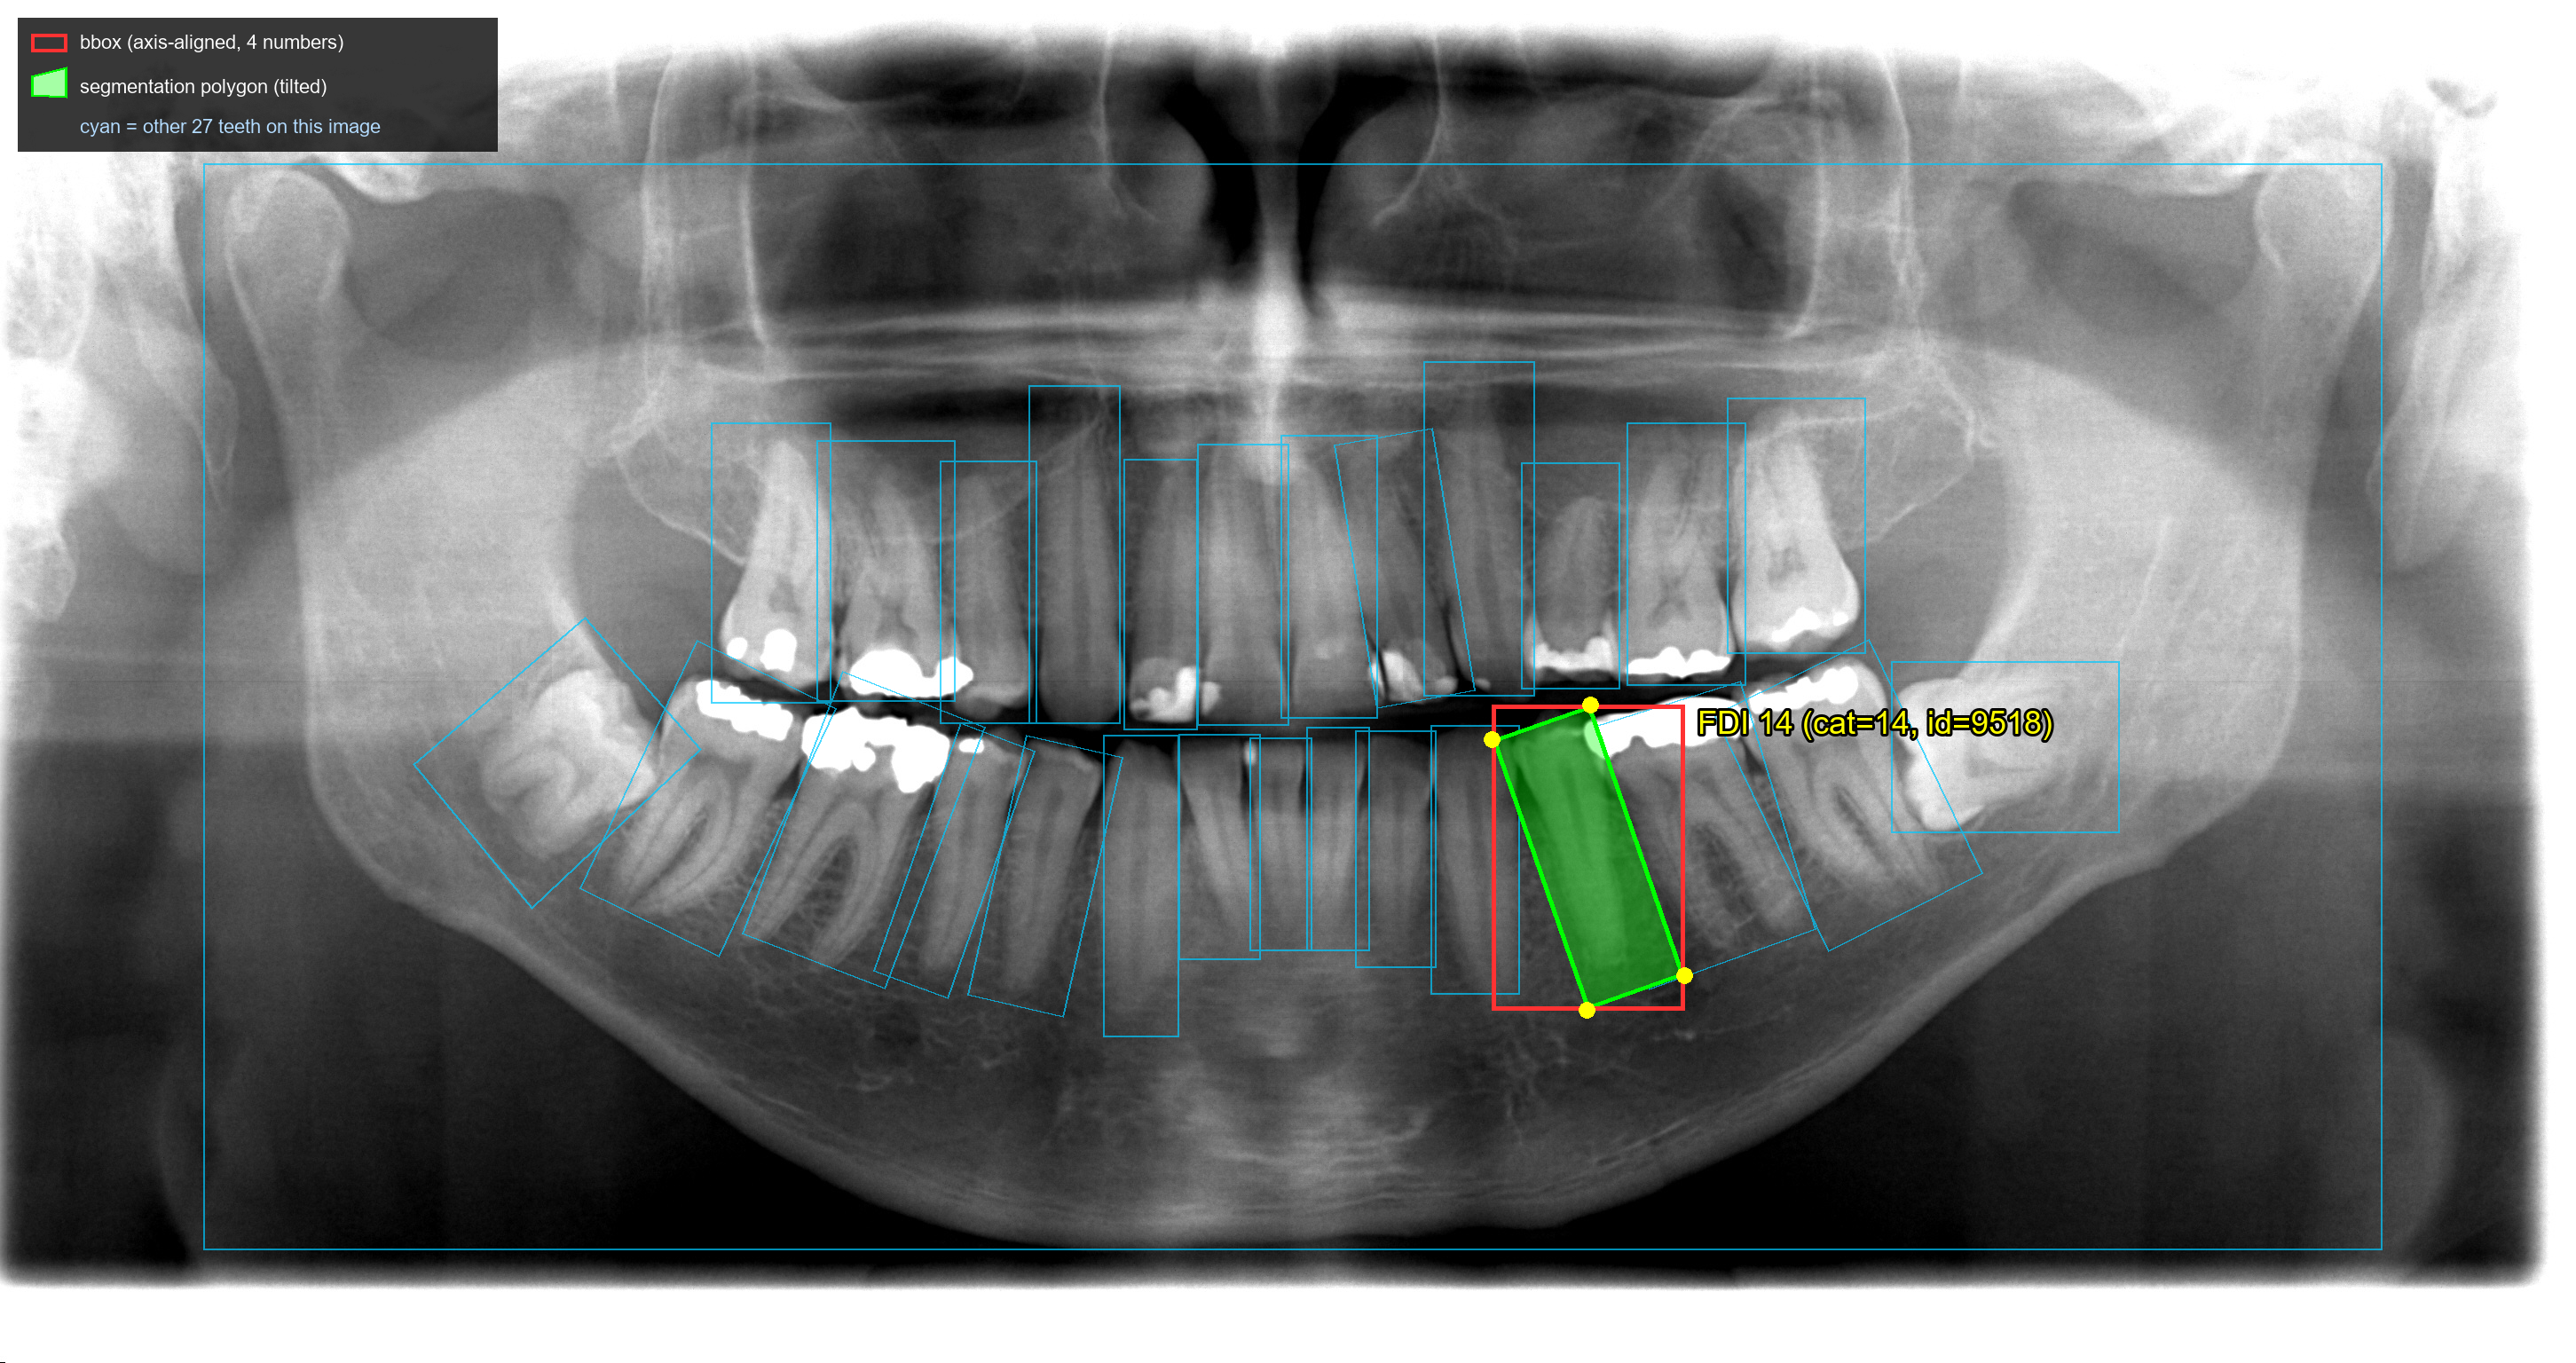
\includegraphics[width=\textwidth]{annotated_example.png}
    \caption{An annotated panoramic image from the PAN924 dataset. Each tooth is marked with an oriented bounding box and its FDI number. The boxes are stored as four-corner polygons (rotated rectangles), not pixel-tight tooth outlines. In the VLM dataset, each tooth is reduced to its FDI number and its condition label.}
    \label{fig:annotated-example}
\end{figure}

The original images are stored in the \texttt{images/} folder. The main annotation file is \texttt{annotations/dataset\_final\_v2.json}. This file is used as the source for the VLM dataset. No new disease labels are created by hand in this step. The labels come from the existing ground-truth annotation file.

The first script in the pipeline is \texttt{build\_5view\_common\_dataset.py}. It reads the original annotations, loads the source images, and builds the common training data. This common dataset is the main dataset of the thesis. The model-specific datasets are created from it later.

For each panoramic image, the pipeline creates five image views:

\begin{itemize}
    \item one full panoramic image;
    \item one upper-left image-space crop;
    \item one upper-right image-space crop;
    \item one lower-left image-space crop;
    \item one lower-right image-space crop.
\end{itemize}

\begin{figure}[h]
    \centering
    \begin{adjustbox}{center, margin=0.5cm 0cm 0cm 0cm}
        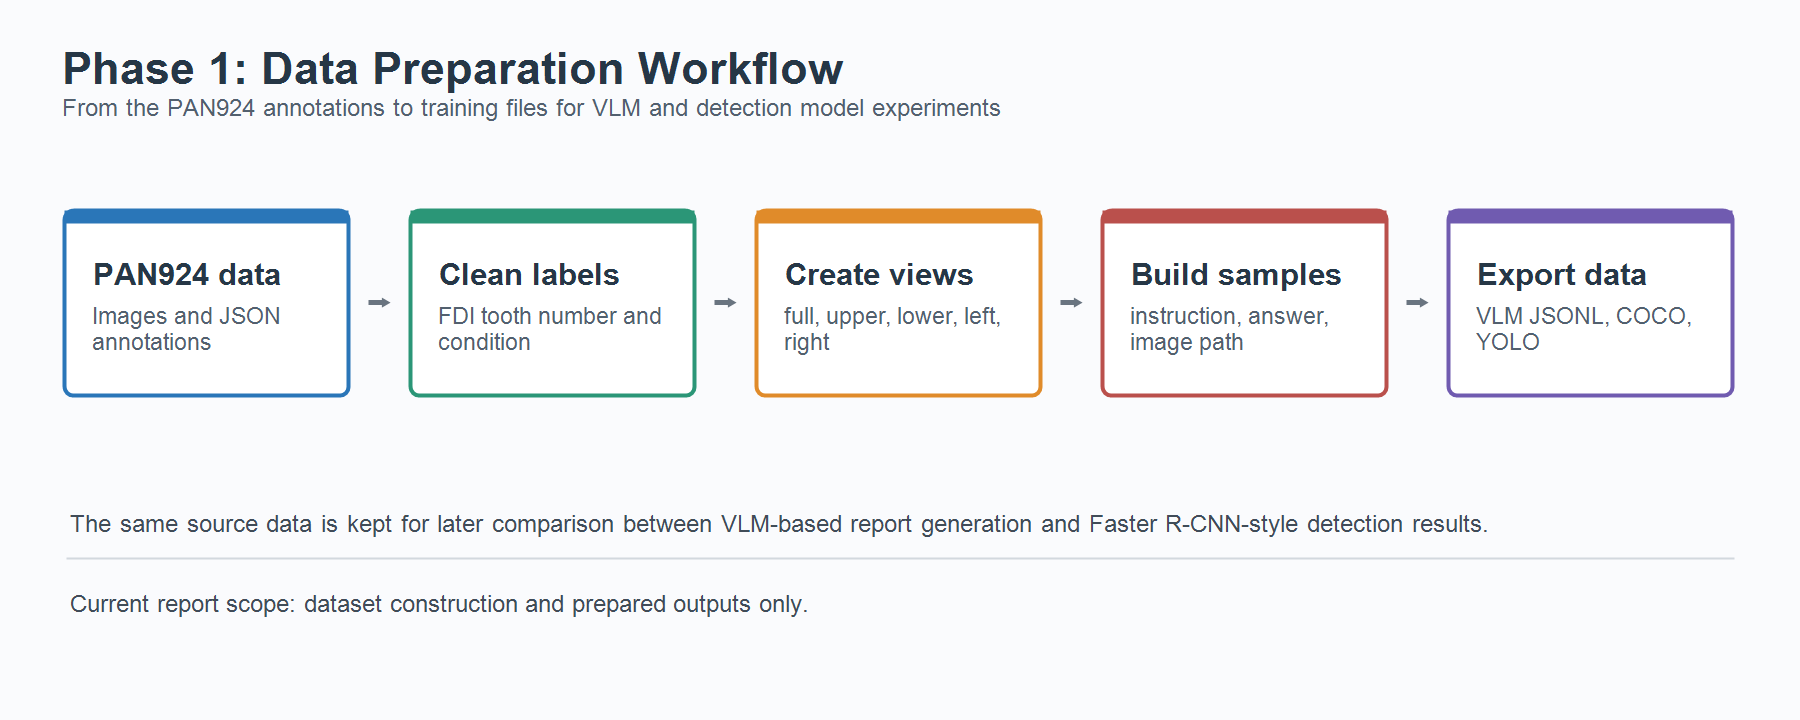
\includegraphics[width=1\textwidth]{phase_1.png}
    \end{adjustbox}
    \caption{Overview of Phase 1: Create image views}
    \label{fig:phase1}
\end{figure}


The regional crops are not random. The split lines are computed from the tooth annotation positions in each image. The left-right split is fixed at the middle of the image. The top-bottom split is not fixed. The script finds the median height of the upper teeth and the median height of the lower teeth. It then cuts halfway between these two heights. This puts the cut between the upper and lower teeth, so it moves with each patient's image instead of sitting at a fixed row.

A 10\% overlap is added along both the horizontal and vertical boundaries of each crop. The main reason is that a tooth sitting exactly on a split line would otherwise be cut in half and appear incomplete. The 10\% margin keeps boundary teeth fully visible in at least one adjacent crop. A smaller overlap, such as 5\%, could still cut these teeth. A larger overlap would make each crop less zoomed-in, so the detail would be less clear.

The region names are image-space names. For example, \texttt{image\_upper\_left} means the upper-left part of the image. It does not mean the anatomical left side of the patient, because a panoramic X-ray is a mirrored view: the patient's right side appears on the image's left.

The five-view design serves two purposes. The full image gives the model global context: it sees all four quadrants together and can observe overall patterns such as missing teeth or widespread caries. The four regional crops zoom into each quadrant and make individual teeth appear larger relative to the image area. This helps the model read fine details such as a small carious lesion or the margin of a crown. Training on both views at the same time means the model learns from both scales in one dataset.

\begin{table}[H]
\centering
\caption{Current PAN924 VLM dataset size}
\begin{tabular}{lccp{5.2cm}}
\toprule
Split & Source images & Samples & Description \\
\midrule
Train & 739 & 3695 & Five views per image \\
Validation & 92 & 460 & Five views per image \\
Test & 93 & 465 & Five views per image \\
\midrule
Total & 924 & 4620 & 924 full reports and 3696 regional reports \\
\bottomrule
\end{tabular}
\end{table}




\subsection{The FDI Tooth Numbering System}

The PAN924 annotations name each tooth with an FDI number. FDI stands for F\'ed\'eration Dentaire Internationale. It is the tooth numbering system used by most dentists around the world. Every tooth gets a two-digit number. The thesis keeps this system, so the model learns to name teeth the same way a dentist does.

The first digit is the quadrant. The mouth is split into four quadrants: upper right, upper left, lower left, and lower right. The sides are read from the patient's point of view, not from the viewer's side. Table~\ref{tab:fdi-quadrant} lists the four quadrants and their number ranges.

\begin{table}[H]
\centering
\caption{The four FDI quadrants (first digit)}
\label{tab:fdi-quadrant}
\begin{tabular}{ccc}
\toprule
First digit & Location (patient's view) & FDI range \\
\midrule
1 & Upper right & 11--18 \\
2 & Upper left  & 21--28 \\
3 & Lower left  & 31--38 \\
4 & Lower right & 41--48 \\
\bottomrule
\end{tabular}
\end{table}

The second digit is the tooth position inside the quadrant. Counting starts at the front center of the mouth and moves toward the back. Position 1 is the central incisor, right next to the midline. Position 8 is the third molar, the wisdom tooth at the very back. Table~\ref{tab:fdi-position} lists the eight positions.

\begin{table}[H]
\centering
\caption{The eight tooth positions (second digit)}
\label{tab:fdi-position}
\begin{tabular}{cl}
\toprule
Second digit & Tooth name \\
\midrule
1 & Central incisor \\
2 & Lateral incisor \\
3 & Canine \\
4 & First premolar \\
5 & Second premolar \\
6 & First molar \\
7 & Second molar \\
8 & Third molar (wisdom tooth) \\
\bottomrule
\end{tabular}
\end{table}

Reading an FDI number is simple. The two digits are read one by one, not as a single number. For example, tooth 36 is read as ``three, six''. The first digit 3 is the lower-left quadrant. The second digit 6 is the first molar. So tooth 36 is the lower-left first molar. In the same way, tooth 11 is the upper-right central incisor, and tooth 48 is the lower-right wisdom tooth.

A full adult mouth has 32 teeth, 8 in each quadrant. Many patients do not have all 32. Wisdom teeth (position 8) are often missing, already removed, or still under the gum. This is one reason why some FDI numbers appear less often in the dataset.

\begin{figure}[H]
    \centering
    \includegraphics[width=0.75\textwidth]{FDI.jpg}
    \caption{The FDI tooth numbering system. Quadrants 1 and 2 are the upper jaw; quadrants 3 and 4 are the lower jaw. Inside each quadrant, the numbers grow from the front center toward the back.}
    \label{fig:fdi}
\end{figure}

\subsection{Stratified Data Split}

The dataset is divided into train, validation, and test. The split is done at the source-image level. All five views of one image (the full image and its four crops) always go to the same split. This matters because the five views show the same mouth. Putting some views in training and others in test would let the model see the test anatomy during training. This is a form of data leakage, and it would make the test results look better than they really are.

The split is also stratified by dental condition. For each image, the script finds the rarest condition that appears in it. It then groups the images by this condition. The 80/10/10 split is applied inside each group. This way, each condition, even a rare one, is spread across train, validation, and test in similar proportions. A plain random split could, by bad luck, send all images of a rare condition to one split.

The order inside each group is set by a hash, not by chance. The script takes the SHA-256 hash of the image filename, together with a fixed seed of 924, and sorts the images by this value. It then cuts the sorted list into 80\%, 10\%, and 10\%. A hash is a fixed-length fingerprint of the text, and the same filename always gives the same hash. So the split is fully reproducible: running the script again gives the exact same result. After this first pass, a small balancing step moves a few images between splits so the final sizes match the targets.

The final split has 739 training images, 92 validation images, and 93 test images, which is about 80/10/10.

\subsection{Common Report Schema and Prompt Templates}

The current pipeline does not build open-ended question-answer data. It builds a common report dataset for VLM training. This is a better fit for the current thesis stage because the output needs to look like a short dental report, not like a question-answer pair.

Each sample is stored as one JSONL row. The row keeps the image path, source image name, view name, task name, prompt, target answer, labels, and metadata. The answer is always stored as valid JSON. This makes the dataset easier to inspect by script and easier to convert later.

There are two task types. The first task is \texttt{full\_quadrant\_report}. It uses the full panoramic image. The target output contains the four image-space regions used in the crop step. Each region has a list of visible annotated teeth, the FDI number, the condition code, the condition name, and one short comment. The full report also has an overall summary.

The second task is \texttt{regional\_report}. It uses one cropped image region. The target output contains the region name, the visible annotated teeth in that crop, and one short comment for the region.

The prompt is kept short on purpose. It tells the model the image type and the JSON schema that must be returned. Long medical instructions are not used at this stage because the first goal is to make a stable dataset. The clinical meaning comes from the ground-truth labels, not from a free-form prompt.

\begin{table}[H]
\centering
\caption{Task types in the common report dataset}
\begin{tabular}{llp{5.6cm}}
\toprule
Task & Image input & Target output \\
\midrule
\texttt{full\_quadrant\_report} & Full panoramic image & Four-region JSON report and summary \\
\texttt{regional\_report} & One regional crop & Tooth list and region comment \\
\bottomrule
\end{tabular}
\end{table}


\subsection{Clinical Text Generation from Ground-Truth Labels}

The report text is generated from the annotation labels. No external AI model or API is used in this step. This is important because the dataset should not add new findings that are not in the original annotations.

The script \texttt{generate\_clinical\_reports.py} reads the raw common JSONL files from the raw subfolder of \texttt{common}. Then it writes the final JSONL files back to \texttt{common}. The script only changes the \texttt{comment} and \texttt{summary} fields. It does not change the image path, split, task name, tooth number, condition label, or JSON structure.

The text generation rule is simple. If a region has abnormal findings, those findings are mentioned first. Teeth with the same condition are grouped together. Healthy teeth are not listed one by one when abnormal teeth already exist. If a region has only healthy annotated teeth, the comment says this clearly. If a region has no annotated teeth, the comment also says this clearly.

For example, if a region contains caries on one tooth and a restoration on another tooth, the generated comment has this style:

\begin{quote}
This region shows caries on tooth 33 and a restoration on tooth 34. The remaining annotated teeth are healthy.
\end{quote}

This text is not used as a final clinical diagnosis. It is used as a training target for report-style VLM output. In a real dental setting, the original X-ray and any generated report must still be checked by a qualified dentist.


\subsection{Validation and Quality Control}

After the common dataset is generated, the validation script checks whether each JSONL row has the required fields. It also checks the image paths, task names, output JSON schema, condition labels, and split information.

For full-image reports, the validator checks that all four region keys are present. It also checks that the target teeth match the saved labels for each region. For regional reports, it checks that the region name and tooth list in the target output match the label fields.

The validation result shows \texttt{ok: true} and \texttt{error\_count: 0}. The final common dataset contains 924 unique source images and 4620 samples. These include 924 full-image report samples and 3696 regional report samples. The split is image-based, so one source image does not appear in more than one split.

Several samples are also inspected manually. This is mainly to see whether the comments match the tooth labels and whether the crops are useful. This manual check is not the same as expert dental review. It is only a practical check for dataset consistency at this stage.


\subsection{Dataset Summary, Label Set, and Class Balancing}

The common dataset is stored in \texttt{vlm\_report\_dataset/common/}. This folder is treated as the main dataset. It contains \texttt{train.jsonl}, \texttt{val.jsonl}, and \texttt{test.jsonl}. It also contains the copied full images, the four regional crops for each image, and metadata files such as the build summary, split report, crop manifest, clinical generation summary, and validation report.

The dataset uses 12 condition codes after label cleaning. Some rare or overlapping labels are remapped before the files are written. For example, \texttt{Ri}, \texttt{RiM}, and \texttt{TeM} are mapped to \texttt{Te}. The label \texttt{I} is mapped to \texttt{M3i}. This keeps the label set easier to handle during training and evaluation.

\begin{table}[H]
\centering
\caption{Dental condition labels used in the final dataset}
\begin{tabular}{ll}
\toprule
Code & Condition name \\
\midrule
\texttt{H} & healthy \\
\texttt{C} & caries \\
\texttt{R} & restored \\
\texttt{Te} & endodontic treatment \\
\texttt{Im} & implant \\
\texttt{Rr} & residual root \\
\texttt{M3i} & impacted third molar \\
\texttt{M3f} & developing third molar \\
\texttt{CpuM} & prosthetic crown \\
\texttt{Dc} & crown destruction \\
\texttt{Di} & incisal or occlusal wear \\
\texttt{P} & pontic \\
\bottomrule
\end{tabular}
\end{table}


\minisection{Class imbalance in the training data}

The dental conditions are not evenly distributed. In the training split, healthy teeth (\texttt{H}) and restorations (\texttt{R}) together make up most of the annotated teeth. Five conditions appear far less often: crown destruction (\texttt{Dc}), implant (\texttt{Im}), pontic (\texttt{P}), residual root (\texttt{Rr}), and developing third molar (\texttt{M3f}). The most extreme gap is large: healthy teeth outnumber crown destruction by roughly forty to one. If the data is used as it is, the model sees these rare conditions only a small number of times, and it can learn to label almost every tooth as healthy or restored without paying a real penalty. Two techniques are used to reduce this effect. The first works on the data and is described next. The second works during training and is described in Section~\ref{sec:loss-weighting}.

\minisection{Oversampling the rare-condition rows}

The first technique oversamples the rare-condition training rows with the script \texttt{rebalance\_common.py}. It does not create new images. It repeats existing samples so that each rare condition appears more often during training. The result is written to \texttt{common\_balanced/}, and this balanced split is the one used for the experiments.

\minisection{Why only regional crops are oversampled}

Only the four regional crop rows are repeated, never the full panoramic report rows. The reason is signal density. A regional crop contains about 11 annotated teeth on average, while a full report contains about 21. If a crop contains one implant, that implant makes up roughly 1/11 of the answer. In a full report, the same implant makes up only 1/21. So repeating a crop gives a stronger learning signal for the rare condition, because the rare finding takes up a larger part of the answer.

\minisection{The multiplier formula}

Each rare condition receives a copy multiplier based on its prevalence in the regional training crops. Let $p_c$ be the fraction of training crop rows that contain at least one instance of condition $c$, and let $p_{\min}$ be the smallest $p_c$ among the five rare conditions. The multiplier for condition $c$ is:

\begin{equation}
m(c) = \min\!\left(8,\; \frac{p_{\min}}{p_c} \times 8\right)
\label{eq:multiplier}
\end{equation}

This formula has three properties. First, the rarest condition always gets the highest multiplier of 8. Second, a less rare condition gets a smaller multiplier. Third, after oversampling, all five rare conditions appear at roughly the same rate in the training set.

Image-level prevalence ($p_c$) is used rather than raw tooth count. One patient can have multiple implants, so using tooth count gives extra weight to patients who happen to have many instances. Prevalence counts each patient once and is a cleaner measure of how common the condition is across the patient population.

\minisection{Why the cap is 8}

Without a cap, a condition appearing in very few images would get a very large multiplier. The model would then see those same few images hundreds of times and memorize them instead of learning the general visual pattern. The cap of 8 limits the risk of overfitting to single patients, while still giving the rare conditions a much stronger signal.

\minisection{Why MAX-combine is used for samples with multiple rare conditions}

Some crops contain more than one rare condition, for example an implant and a residual root in the same quadrant. Multiplying the two multipliers together ($8 \times 3.97 \approx 32$) would create too many copies of that crop. Instead, the copy count for that crop is set to the maximum of its individual multipliers ($\max(8, 3.97) = 8$). This limits the total growth while still giving each rare condition enough coverage.

\begin{table}[H]
\centering
\caption{Oversampling of the rare conditions in the training split}
\begin{tabular}{llccc}
\toprule
Code & Condition & Multiplier & Teeth before & Teeth after \\
\midrule
\texttt{Dc}  & crown destruction      & 7.89 & 174 & 981 \\
\texttt{Im}  & implant                & 8.00 & 199 & 1081 \\
\texttt{P}   & pontic                 & 4.00 & 362 & 1178 \\
\texttt{Rr}  & residual root          & 3.97 & 332 & 1109 \\
\texttt{M3f} & developing third molar & 3.34 & 398 & 959 \\
\bottomrule
\end{tabular}
\end{table}

After balancing, the training split grows from 3695 to 5817 rows. This is about 57\% more rows. The validation and test splits do not change. Table~\ref{tab:balance-rows} shows the sample counts.

\begin{table}[H]
\centering
\caption{Sample counts before and after balancing}
\label{tab:balance-rows}
\begin{tabular}{lcc}
\toprule
Split & Before balancing & After balancing \\
\midrule
Train & 3695 & 5817 \\
Validation & 460 & 460 \\
Test & 465 & 465 \\
\bottomrule
\end{tabular}
\end{table}

The balanced training split, with 5{,}817 rows, is the one used to fine-tune the models in this work. The validation and test splits stay at their original sizes, so the models are always scored on the true class distribution. This oversampling is only the first half of the imbalance handling; the second half is a loss change applied during training, which is described in Section~\ref{sec:loss-weighting}.


\section{Methods}
\label{sec:methods}

The methods cover four things: the pipeline that turns an image into a report, the five models compared in this work, how each model is adapted for the dental task, and how the class imbalance is handled during training. The five models are Qwen2.5-VL in two sizes (7B and 3B), InternVL3, Phi-3.5-vision, and PaliGemma~2. They are chosen to span different designs, so the comparison can show which design choices matter for reading small teeth.

\subsection{Pipeline}
\label{sec:pipeline}

This subsection describes how a trained model turns a panoramic X-ray into a report at inference time. The pipeline has four stages, and Figure~\ref{fig:pipeline} shows them end to end.

In the first stage, the panoramic image is prepared in the same way as during training. The full image is used for the full-report task, and the four regional crops are used for the regional-report task, with the crop boundaries computed from the tooth positions as described in Section~\ref{sec:materials}. In the second stage, the image is passed through the vision encoder, which turns it into a sequence of image tokens, and a small connector maps those tokens into the language model's input space. In the third stage, the language model reads the image tokens together with the text prompt, which states the image type and the exact JSON schema to return, and it writes the answer one token at a time. In the fourth stage, the generated text is parsed as JSON, and the tooth list, the condition codes, and the short comments are read out. The same parsed structure is what the evaluation script compares against the gold report.

\begin{figure}[H]
    \centering
    % Upload the pipeline diagram as pipeline.png
    \includegraphics[width=\textwidth]{pipeline.png}
    \caption{The vision-language report-generation pipeline. A panoramic image (full view or regional crop) is encoded into image tokens, a connector maps them into the language model, the language model reads the tokens and the schema prompt and generates a JSON report, and the JSON is parsed into tooth-level findings for evaluation.}
    \label{fig:pipeline}
\end{figure}

The same pipeline is used for every model in the study. Only the three internal parts change between models: the vision encoder, the connector, and the language model. The prompt, the JSON schema, and the parsing step stay the same. This is what makes the comparison fair, because the models receive the same input and are asked for the same output.

\subsection{Model Selection and Comparison Design}

The goal is a fair comparison, so the study is set up like a controlled experiment. The model is the only thing that changes. Everything else is kept the same: the same training data, the same data split, the same LoRA settings, and the same evaluation script. Because of this, any difference in the results can be linked to the model, not to a different setup.

The five models are not picked at random. They are chosen to cover four design choices that could matter for reading small teeth in a panoramic X-ray:

\begin{itemize}
    \item \textbf{Vision encoder:} the set spans a native dynamic-resolution ViT, SigLIP, InternViT, and CLIP.
    \item \textbf{Language model family:} the set spans Qwen, Phi, and Gemma.
    \item \textbf{Model size:} the set ranges from about 3B to about 8B parameters.
    \item \textbf{Image handling:} most models keep a large or native image size, while one (PaliGemma~2) uses a fixed 448-pixel input.
\end{itemize}

With this spread, the comparison can show which design choices help most on this task. The model size is tested directly. Two sizes of Qwen2.5-VL are included, the 7B and the 3B, and they share the same architecture. So a 7B-versus-3B comparison shows the effect of size on its own, with everything else held fixed. The comparison can also hint at whether keeping the full image resolution helps the model read small findings.

Three more practical reasons guided this choice. First, all five are well-known open models with public weights. This makes the work easy to reproduce. It also lets us fine-tune the models ourselves, which a closed model behind an API usually does not allow. Second, all five are instruction-tuned, so they can already follow a prompt and return JSON. Third, all five are small enough, about 3B to 8B, to fine-tune on a single GPU with LoRA. Much larger models, such as 72B versions, would not fit on the hardware used here.

\subsection{Shared Architecture}

All five models follow the same basic design, even though the details differ. A vision-language model has three parts. The first part is a vision encoder. It is usually a Vision Transformer (ViT). It reads the image and turns it into a sequence of image tokens. The second part is a connector, often a small multi-layer perceptron (MLP). It maps the image tokens into the same space that the language model uses for words. The third part is a language model. It reads the image tokens and the text prompt together, and then writes the answer one token at a time.

The main differences between the five models are: which vision encoder they use, which language model they use, how large they are, and how they handle a high-resolution image. Table~\ref{tab:vlm-summary} compares the five models on these points.

\begin{table}[H]
\centering
\caption{The five candidate vision-language models}
\label{tab:vlm-summary}
\begin{tabular}{lllll}
\toprule
Model & Vision encoder & Language model & Size & Image handling \\
\midrule
Qwen2.5-VL-7B      & native dynamic ViT   & Qwen2.5 (7B)      & $\sim$8B  & native resolution \\
Qwen2.5-VL-3B      & native dynamic ViT   & Qwen2.5 (3B)      & $\sim$3B  & native resolution \\
InternVL3-8B       & InternViT-300M       & Qwen2.5 (7B)      & $\sim$8B  & 448px tiles \\
Phi-3.5-vision     & CLIP ViT-L/14        & Phi-3.5-mini (3.8B) & $\sim$4.2B & dynamic cropping \\
PaliGemma~2 (3B)   & SigLIP-So400m        & Gemma~2 (2B)      & $\sim$3B  & fixed 448px \\
\bottomrule
\end{tabular}
\end{table}

A high-resolution panoramic X-ray matters here. The teeth are small and close together. A model that can keep more image detail has a better chance to read each tooth. This is why the image-handling column is important for this task. Four of the five models can take a larger or native image size. Only PaliGemma~2 uses a fixed 448-pixel input.

\subsection{The Five Models}

Each model is described in short below. The checkpoint name is the exact version used in this project, and the citation points to its paper or model card. The figures show the architecture of each model.

\minisection{Qwen2.5-VL-7B-Instruct (Alibaba)}

Checkpoint: \texttt{Qwen/Qwen2.5-VL-7B-Instruct} \cite{qwen25vl2025}. Its vision encoder is a ViT with native dynamic resolution, so the image is not forced to a fixed size and small details are kept. The language model is the Qwen2.5 decoder (about 7B). This is the strongest general model in the set.

\begin{figure}[H]
    \centering
    % Upload the Qwen2.5-VL architecture figure as qwen_arch.png
    \includegraphics[width=0.85\textwidth]{qwen_arch.png}
    \caption{Architecture of Qwen2.5-VL: a native dynamic-resolution ViT feeds image tokens into the Qwen2.5 language model.}
    \label{fig:qwen-arch}
\end{figure}

\minisection{Qwen2.5-VL-3B-Instruct (Alibaba)}

Checkpoint: \texttt{Qwen/Qwen2.5-VL-3B-Instruct} \cite{qwen25vl2025}. This is the smaller version of the same Qwen2.5-VL family. It keeps the native dynamic-resolution ViT, but pairs it with a smaller Qwen2.5 language model (about 3B). It is included for one reason: to measure the effect of model size. Because it shares the architecture of the 7B model, a direct 7B-versus-3B comparison shows whether the extra parameters are worth the higher cost on this task. The architecture is the same as in Figure~\ref{fig:qwen-arch}, only the language model is smaller.

\minisection{InternVL3-8B (OpenGVLab)}

Checkpoint: \texttt{OpenGVLab/InternVL3-8B} \cite{zhu2025internvl3}. It follows a ViT--MLP--LLM design, with an InternViT-300M encoder and a Qwen2.5 language model (about 7B). It cuts a large image into 448-pixel tiles and uses a pixel unshuffle step to keep the token count low, which helps with tiny findings.

\begin{figure}[H]
    \centering
    % Upload the InternVL3 architecture figure as internvl_arch.png
    \includegraphics[width=0.85\textwidth]{internvl_arch.png}
    \caption{Architecture of InternVL3: the ViT--MLP--LLM pattern with InternViT-300M, a two-layer MLP, and the Qwen2.5 language model. Pixel unshuffle reduces the token count per tile.}
    \label{fig:internvl-arch}
\end{figure}

\minisection{Phi-3.5-vision-instruct (Microsoft)}

Checkpoint: \texttt{microsoft/Phi-3.5-vision-instruct} \cite{abdin2024phi3}. It is one of the smaller models, about 4.2B in total, with a CLIP ViT-L/14 encoder and the Phi-3.5-mini language model (3.8B). It uses dynamic cropping for high-resolution input, and its small size needs less GPU memory.

\minisection{PaliGemma~2 (3B, 448px) (Google)}

Checkpoint: \texttt{google/paligemma2-3b-pt-448} \cite{steiner2024paligemma2}. It uses a SigLIP-So400m encoder, a single linear projection, and a Gemma~2 language model (about 2B), for about 3B in total. It differs from the others in two ways: it uses a fixed 448-pixel image size, and it is a prefix-LM, where the image and the prompt attend to each other freely. It is a gated model, so its license must be accepted before download.

\begin{figure}[H]
    \centering
    % Upload the PaliGemma 2 architecture figure as paligemma_arch.png
    \includegraphics[width=0.85\textwidth]{paligemma_arch.png}
    \caption{Architecture of PaliGemma~2: a SigLIP-So400m encoder with a linear projection feeds image tokens into the Gemma~2 language model, which uses a prefix-LM attention pattern.}
    \label{fig:paligemma-arch}
\end{figure}

\subsection{Model Adaptation with LoRA and QLoRA}
\label{sec:lora}

All five models are large, from about 3 to 8 billion parameters. Training every weight would need a lot of GPU memory and a lot of data. The dental dataset is small, so full fine-tuning is not a good fit. It would be slow and would overfit easily. For these reasons the models are not fully retrained. They are adapted with QLoRA on a single 24~GB GPU, which keeps the frozen base model in 4-bit and trains only small low-rank adapters.

\minisection{LoRA: low-rank adaptation}

LoRA keeps all the original model weights frozen. It does not change them at all. Instead, it adds a small trainable update next to each weight matrix. The idea behind LoRA is that the change needed to fit a new task is ``low-rank''. This means the change can be written as the product of two thin matrices instead of one large one.

Take an original weight matrix $W$ of size $d \times k$. LoRA adds two small matrices: $A$ of size $r \times k$ and $B$ of size $d \times r$. The number $r$ is the rank, and it is small (here $r = 8$). During the forward pass, the layer output becomes:

\begin{equation}
h = Wx + \frac{\alpha}{r}\, BAx
\label{eq:lora}
\end{equation}

The matrix $W$ stays frozen, and only $A$ and $B$ are trained. The term $\alpha/r$ is a fixed scaling factor that sets how strong the update is. Because $r$ is small, $A$ and $B$ together hold far fewer numbers than $W$. This drops the trainable weights from billions to only a few million.

\begin{figure}[H]
    \centering
    % Upload a LoRA / QLoRA diagram as qlora_arch.png
    \includegraphics[width=0.7\textwidth]{qlora_arch.png}
    \caption{LoRA adaptation. The original weight $W$ is frozen (in QLoRA it is stored in 4-bit). Only the two low-rank matrices $A$ and $B$ are trained, and their output is added to the frozen path.}
    \label{fig:qlora-arch}
\end{figure}

\minisection{QLoRA: LoRA on a 4-bit base}

QLoRA adds one more step on top of LoRA. Before training, the frozen base model is loaded in 4-bit instead of the usual 16-bit. This is done with the BitsAndBytes library, using the NF4 (4-bit NormalFloat) format. Storing the base weights in 4-bit cuts their memory by about four times. The small LoRA matrices $A$ and $B$ are still kept in bfloat16, so the trained part stays precise.

The 4-bit weights are only used to run the frozen base forward. They are never updated. All the learning happens in the bfloat16 LoRA matrices. This is why a 4-bit base does not hurt training much: the precision that matters for the gradient updates is kept in the adapter. Thanks to this, even the 8B model fits on one 24~GB GPU.

\minisection{What is trained and what is frozen}

LoRA is applied to all linear layers of the language model (the setting \texttt{target\_modules = all-linear}). The vision encoder is frozen and gets no LoRA, because it is already pretrained on large image data and the dental set is too small to retrain it safely. So the only trained parts are the LoRA matrices on the language-side linear layers. Everything else keeps its original values.

\minisection{Training hardware}

All five models are trained on a single NVIDIA L4 GPU with 24~GB of memory. At this size, a 7--8B model in 16-bit does not fit together with the image activations, so QLoRA is required: the frozen base is loaded in 4-bit, while the LoRA adapters stay in bfloat16. This is what lets even the 8B model train on one 24~GB card. The same QLoRA recipe is used for every model, so the comparison stays fair.

This same method is used for all five models. The exact values, such as the rank, the alpha, and the learning rate, are listed in the Experimental Setup chapter. Using one shared method means the comparison between the models is fair: any difference in results comes from the models themselves, not from different training tricks.

\subsection{Handling Class Imbalance at Training Time}
\label{sec:loss-weighting}

Oversampling (Section~\ref{sec:materials}) helps, but it has a clear limit. Every report, even one that contains a rare implant, is still mostly made of healthy and restored teeth. When a rare-condition report is repeated, those common teeth are repeated with it. As a result, the rare-to-common ratio only improves so far, and the rarest conditions are still a small share of the training signal.

The second technique works directly on the loss instead of the data. A vision-language model is trained with token-level cross-entropy: at each position it is penalised by how wrong its predicted next token is, and every token counts the same. The condition codes that name a rare disease, such as \texttt{Dc} or \texttt{Rr}, are only a tiny fraction of all the tokens in a report, so getting them wrong barely changes the average loss. The model can reach a low loss while still labelling almost every tooth as healthy or restored.

To counter this, the loss on the tokens that spell a rare condition code is multiplied by a fixed weight (here, three), while every other token keeps a weight of one. The rare codes are the same five used earlier: \texttt{Dc}, \texttt{Im}, \texttt{P}, \texttt{Rr}, and \texttt{M3f}. In practice, the token ids that make up these codes are read from each model's tokenizer once, and the training loss is scaled up whenever the target token is one of them. The penalty for mislabelling a rare tooth is now three times larger, so the model can no longer ignore these conditions cheaply.

The two techniques are complementary. Oversampling increases how often a rare condition is seen, and the loss weighting increases how much each rare token matters when it is seen. Both are used together for every model, and both leave the validation and test data untouched, so the reported scores still reflect the true class distribution.

\subsection{Dataset Conversion for the Model Families}

The common dataset is model-independent. After it is validated, a conversion script writes the same data into model-specific folders. This keeps the source data fixed while letting each model read the data in the format it expects.

Converted files are prepared for the four families used in this work: Qwen, InternVL, Phi, and PaliGemma. Every converted folder keeps the same split, with 5{,}817 training rows (the balanced split), 460 validation rows, and 465 test rows. Because the split is identical, the models can be trained and tested on exactly the same data.

The conversion changes only the outer data format. Qwen uses a message format with an image list, InternVL uses conversation-style rows, Phi uses a prompt-and-response format, and PaliGemma uses prefix and suffix fields. The image paths, the target report content, the split names, and the metadata all still come from the common dataset, so the models differ only in their wrapper, not in what they are asked to learn.

\chapter{Experimental Setup}

This chapter describes how the five models are trained and evaluated. Every model uses the same data, the same settings, and the same evaluation script, so any difference in the results can be linked to the model and not to the setup.

\section{Training Environment and Execution}

All five models are fine-tuned with QLoRA on a single NVIDIA L4 GPU with 24~GB of memory. Training is run with the ms-swift framework, which loads the base model from Hugging Face, applies the 4-bit quantization and the LoRA adapters, and runs the training loop. A full run takes several hours, so each one is started inside a terminal multiplexer (tmux) on the server. The job then keeps running even if the connection drops or the laptop is closed, and it can be checked again later.

Two safeguards reduce wasted time on the GPU. First, every new model is started with a short five-step trial run before the full run. If the model loads, quantizes, and trains for five steps without running out of memory, the configuration is sound and the full run is started. This catches a broken setting in about two minutes instead of after several hours. Second, a checkpoint is saved every 100 steps, so if a run stops for any reason it can continue from the last checkpoint instead of starting over.

\section{Training Configuration}

The models are adapted with QLoRA, and how LoRA and QLoRA work is explained in Section~\ref{sec:lora}. This section only lists the exact settings. Only three things change between models: the model name, the output folder, and, for the models that support it, the image-resolution option. Everything else is shared.

\minisection{LoRA rank and alpha}

The rank is set to 8. A lower rank means fewer trainable parameters and less risk of overfitting on a small dataset. Rank 8 is a common choice for 7B models. It is large enough to learn the task, but still small. The alpha is set to 32. In the LoRA update, the added weights are scaled by $\alpha / r$, which is $32 / 8 = 4$ here. This factor sets how strongly the update changes the output. A value of 4 gives a clear learning signal without changing the frozen weights too much.

\minisection{Why the vision encoder is frozen}

Each VLM has a vision encoder (a ViT-based model) that converts the input image into feature vectors. This encoder is already pretrained on a huge amount of image data, so its features are good. The dental set has only a few thousand training views. That is too small to retrain the encoder safely, and training it could harm its general features. So it is kept frozen. Only the language-side adapter learns to read the dental features, which is more stable.

\minisection{Gradient accumulation}

The per-device batch size is 1 because loading a 7B model with an image leaves very little GPU memory for storing multiple samples at once. Gradient accumulation is set to 16, so gradients from 16 consecutive forward passes are summed before one weight update. This gives an effective batch size of 16 without needing 16 samples in memory at the same time. A larger effective batch size makes the gradient estimate less noisy and often leads to more stable training.

\begin{table}[H]
\centering
\caption{Training hyperparameters shared by all five models}
\begin{tabular}{ll}
\toprule
Setting & Value \\
\midrule
Fine-tuning method      & QLoRA (4-bit base, bfloat16 adapters) \\
Quantization            & 4-bit NF4, double quantization, bfloat16 compute \\
LoRA rank               & 8 \\
LoRA alpha              & 32 \\
LoRA dropout            & 0.1 \\
Target modules          & all linear layers \\
Vision encoder          & frozen \\
Training split          & balanced (5{,}817 rows) \\
Rare-token loss weight  & 3.0 \\
Epochs                  & 2 (best checkpoint chosen by validation loss) \\
Learning rate           & 1e-4 \\
LR scheduler            & cosine \\
Warmup ratio            & 0.05 \\
Weight decay            & 0.1 \\
Batch size per device   & 1 \\
Gradient accumulation   & 16 (effective batch size 16) \\
Max sequence length     & 4096 \\
Max image pixels        & 401{,}408 \\
Eval / save interval    & every 100 steps \\
Random seed             & 924 \\
\bottomrule
\end{tabular}
\end{table}

\section{Checkpoint Selection}

A checkpoint is saved every 100 steps, and the last checkpoint is not always the best one, because a model can start to overfit near the end of training. The validation loss is recorded at every save point, so the checkpoint with the lowest validation loss is selected for the final test. This selection is cheap, because the validation loss is already computed during training and needs no extra generation. The chosen checkpoint is the only one run on the test set.

\section{Evaluation Metrics}

\minisection{Generating the predictions}

For evaluation, the selected checkpoint is run on the 465 test rows. Each image is given the same schema prompt used in training, and decoding is greedy (temperature set to zero) so the output is reproducible. The generation length is capped at 1{,}280 tokens, which is enough for the longest report in the data, so no report is cut off before it ends. The text the model returns is then parsed as JSON and passed to the scoring script.

The evaluation uses one script, \texttt{eval\_report.py}, for all models. It compares the predicted JSON report with the gold JSON report. The basic unit is one tooth in one region. For each unit, the script checks the FDI number and the condition label.

The metrics are grouped in a simple way. The detection metrics ask if the model finds the right teeth. The classification metrics look at whether a found tooth has the correct condition. The joint metrics combine the two. The last group checks the text quality and the JSON format. Table~\ref{tab:eval-metrics} lists the groups.

\begin{table}[H]
\centering
\caption{Groups of evaluation metrics}
\label{tab:eval-metrics}
\begin{tabular}{lp{8.5cm}}
\toprule
Group & What it measures \\
\midrule
Detection      & Whether the right teeth are found by FDI number: precision, recall, F1, plus the rate of invented teeth and missed teeth. \\
Classification & For a tooth that is found, whether the condition is correct: per-condition and averaged precision, recall, and F1. \\
Joint          & Whole-tooth accuracy, where the FDI number and the condition are both correct, and the exact report match rate. \\
Generation     & The share of outputs that are valid JSON, and the ROUGE-L score on the comment and summary text. \\
\bottomrule
\end{tabular}
\end{table}

These metrics cover both parts of the task. The detection and classification metrics show if the model finds the correct dental findings. The generation metrics show if the output is valid and readable. The detection and classification metrics can also be used for the Faster R-CNN baseline, so the recognition part can be compared on the same ground.

\minisection{ROUGE-L}

ROUGE-L measures text similarity using the Longest Common Subsequence (LCS) between two strings. LCS finds the longest sequence of tokens that appears in both the predicted text and the reference text in the same order, but the tokens do not have to be adjacent. For example, if the reference is ``caries on tooth 33 and restoration on tooth 35'' and the prediction is ``tooth 33 caries, tooth 35 restored'', ROUGE-L will find a long common subsequence even though the word order is slightly different.

ROUGE-L is more appropriate for dental report text than ROUGE-1 or ROUGE-2, because it captures word-order similarity without requiring exact adjacent matches. A report that lists the correct tooth numbers and condition names in the right order scores high. A report that uses wrong numbers or invents conditions that do not exist scores low.

The ROUGE-L score is computed from scratch in \texttt{eval\_report.py} using the standard LCS dynamic programming algorithm, without relying on external libraries. This makes the evaluation code self-contained and easy to reproduce.

\minisection{Detection and classification metrics}

Precision, recall, and F1 are computed at the tooth level. For detection, a predicted tooth is a true positive if its FDI number matches a gold tooth in the same region. Precision measures how many predicted teeth are correct; recall measures how many gold teeth were found. For classification, the same tooth-level matching is used, and a predicted condition is correct only if it matches the gold condition exactly. Per-condition F1 is also reported so that rare-condition performance is visible separately from the overall average.

\minisection{Hallucination and miss rates}

Two additional metrics are reported alongside detection. The hallucination rate is the fraction of predicted teeth that do not match any gold tooth; these are invented findings. The miss rate is the fraction of gold teeth that the model did not predict. Both rates are important for a dental support tool: a model that invents many findings could mislead the dentist, and a model that misses many findings is not useful as a draft report.

\minisection{Per-condition and per-tooth breakdowns}

Two averages are reported for the classification metrics. The micro average pools every tooth together, so it is driven by the common conditions. The macro average takes the mean over the conditions, so each condition counts the same, and a model that ignores the rare conditions is punished here. Because the rare conditions are the hard part of this task, the macro F1 is treated as the headline metric, and the per-condition F1 is also reported so that each rare condition can be read on its own.

Two visual summaries support the tables. The first is a confusion matrix between the gold and predicted conditions, which shows where the model mixes up conditions, for example labelling a rare condition as healthy. The second is a per-tooth detection chart laid out like a dental chart, which shows the recall for each FDI position and makes it easy to see whether certain teeth, such as the wisdom teeth, are missed more often. Both are produced for every model in the Results chapter.

\chapter{Results}

This chapter reports the results of the five models on the held-out test set of 465 rows. All models use the same checkpoint-selection rule and the same evaluation script, so the numbers can be compared directly. The per-tooth chart and the confusion matrix are shown for the best model, InternVL3, while the tables cover all five models.

\section{Overall Comparison}

Table~\ref{tab:results-recognition} reports the recognition metrics, and Table~\ref{tab:results-text} reports the error rates and the text quality. The macro F1 is the headline number, because it gives each condition the same weight and therefore reflects how well the rare conditions are handled. The FDI detection F1 shows whether the model finds the right teeth, and the tooth accuracy shows whether it gets both the tooth and its condition right at the same time.

\begin{table}[H]
\centering
\caption{Recognition results on the test set: tooth detection (FDI) and condition classification (higher is better)}
\label{tab:results-recognition}
\small
\begin{adjustbox}{max width=\textwidth}
\begin{tabular}{lcccccc}
\toprule
& \multicolumn{3}{c}{Detection (FDI)} & \multicolumn{2}{c}{Classification} & Joint \\
\cmidrule(lr){2-4}\cmidrule(lr){5-6}\cmidrule(lr){7-7}
Model & Precision & Recall & F1 & Macro F1 & Micro F1 & Tooth acc. \\
\midrule
Qwen2.5-VL-7B      & \textbf{0.779} & 0.846 & 0.811 & 0.152 & 0.537 & 0.452 \\
Qwen2.5-VL-3B      & 0.765 & 0.891 & 0.823 & 0.139 & 0.553 & 0.470 \\
InternVL3-8B       & 0.776 & 0.892 & \textbf{0.830} & \textbf{0.189} & \textbf{0.607} & \textbf{0.519} \\
Phi-3.5-vision     & 0.721 & 0.895 & 0.799 & 0.102 & 0.461 & 0.383 \\
PaliGemma~2 (3B)   & 0.768 & \textbf{0.901} & 0.830 & 0.174 & 0.606 & 0.518 \\
\bottomrule
\end{tabular}
\end{adjustbox}
\end{table}

\begin{table}[H]
\centering
\caption{Error rates and text quality on the test set}
\label{tab:results-text}
\small
\begin{tabular}{lccccc}
\toprule
Model & Hallucination & Miss rate & Exact report & ROUGE-L & Valid JSON (\%) \\
\midrule
Qwen2.5-VL-7B      & \textbf{0.221} & 0.154 & 0.125 & 0.654 & 100 \\
Qwen2.5-VL-3B      & 0.235 & 0.109 & 0.120 & 0.663 & 100 \\
InternVL3-8B       & 0.224 & 0.108 & 0.133 & 0.696 & 100 \\
Phi-3.5-vision     & 0.279 & 0.105 & 0.127 & 0.603 & 99.6 \\
PaliGemma~2 (3B)   & 0.232 & \textbf{0.099} & \textbf{0.136} & \textbf{0.697} & 100 \\
\bottomrule
\end{tabular}
\end{table}

The recognition results split into two clear levels. InternVL3-8B is the best model overall. It has the highest macro F1 (0.189), micro F1 (0.607), and tooth accuracy (0.519). PaliGemma~2 follows very closely, even though it is the smallest model and uses a fixed 448-pixel input. Qwen2.5-VL comes next, and Phi-3.5-vision is last on every recognition metric.

There are two main points here. First, model size is not the main factor. PaliGemma~2 (about 3B) almost matches InternVL3 (about 8B), and the 3B Qwen is close to the 7B Qwen, even slightly higher on micro F1 and tooth accuracy. So a larger model is not automatically better on this task. Second, the FDI detection F1 is high for every model (0.80 to 0.83), but the tooth accuracy is much lower (0.38 to 0.52). This gap means the hard part is not finding the teeth, but naming the correct condition.

The detection numbers also show how the models behave. For every model the FDI recall (0.85 to 0.90) is higher than the FDI precision (0.72 to 0.78). So the models find most of the real teeth, but they also report some teeth that are not in the gold report. This is the same effect as the hallucination rate being higher than the miss rate in Table~\ref{tab:results-text}. The fixed-resolution PaliGemma~2 detects teeth as well as the native-resolution models, and it even has the highest recall, so keeping the native image size did not give a clear detection gain here.

Figure~\ref{fig:model-comparison} shows the same comparison as a bar chart. It makes two things easy to see at a glance: the FDI detection bars are high and similar for every model, while the macro F1 bars are low for all of them. The hard part of the task is therefore the condition, not the tooth.

\begin{figure}[H]
    \centering
    % Produced by the metrics-plotting script from the per-model metrics JSON files.
    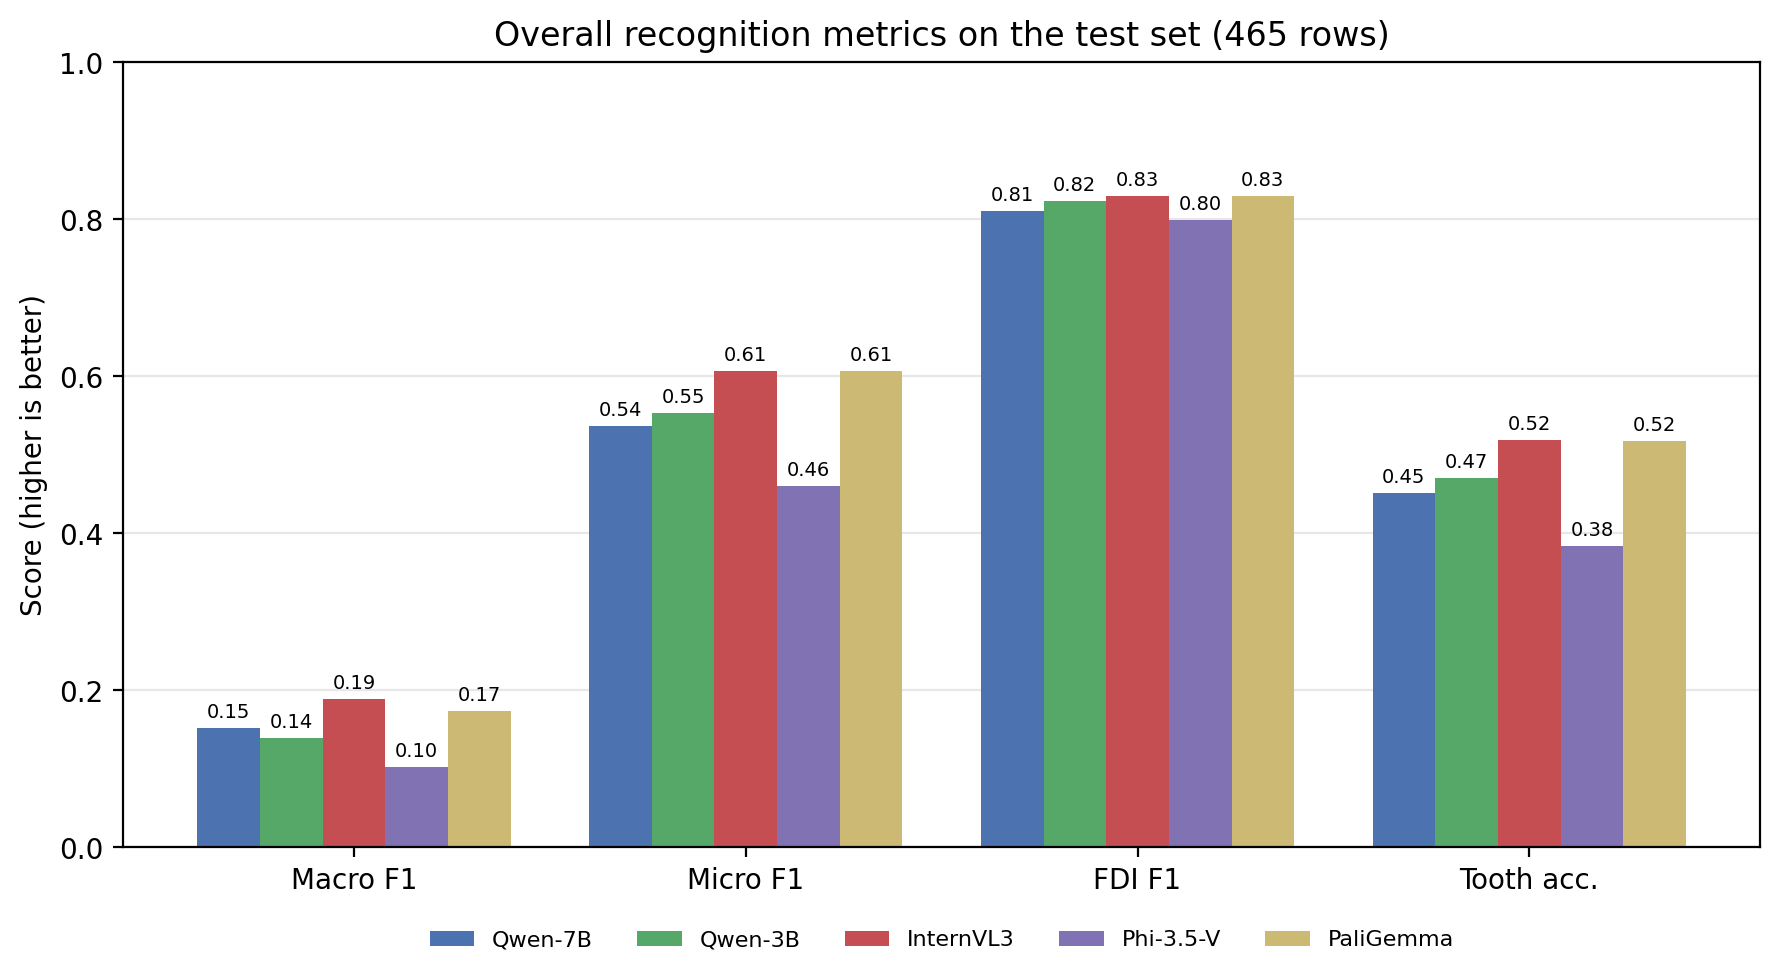
\includegraphics[width=\textwidth]{model_comparison_bars.png}
    \caption{Overall recognition metrics for the five models on the test set (465 rows). InternVL3-8B is highest on macro F1, micro F1, and tooth accuracy; PaliGemma~2 is a close second despite being the smallest model. FDI detection is high and similar for all models, while the macro F1 stays low, which shows that condition classification, not tooth detection, is the hard part.}
    \label{fig:model-comparison}
\end{figure}

\section{Per-Condition Results}

Table~\ref{tab:results-percond} reports the per-condition F1 for every model. The support column is the number of test teeth for each condition, and it is the same for all models because it comes from the gold labels. The five rare conditions (\texttt{Dc}, \texttt{Im}, \texttt{P}, \texttt{Rr}, \texttt{M3f}) are the ones most affected by the class imbalance, so they are the most important rows to read.

\begin{table}[H]
\centering
\caption{Per-condition F1 on the test set}
\label{tab:results-percond}
\small
\begin{adjustbox}{max width=\textwidth}
\begin{tabular}{llcccccc}
\toprule
Code & Condition & Support & Qwen-7B & Qwen-3B & InternVL & Phi & PaliGemma \\
\midrule
\texttt{H}    & healthy                & 3788 & 0.724 & 0.729 & 0.765 & 0.683 & 0.762 \\
\texttt{R}    & restored               & 1712 & 0.419 & 0.426 & 0.495 & 0.274 & 0.474 \\
\texttt{Te}   & endodontic treatment   & 267  & 0.107 & 0.093 & 0.104 & 0.000 & 0.079 \\
\texttt{C}    & caries                 & 158  & 0.032 & 0.000 & 0.026 & 0.026 & 0.000 \\
\texttt{Di}   & incisal/occlusal wear  & 129  & 0.028 & 0.040 & 0.000 & 0.000 & 0.104 \\
\texttt{CpuM} & prosthetic crown       & 114  & 0.110 & 0.044 & 0.180 & 0.075 & 0.048 \\
\texttt{M3i}  & impacted third molar   & 84   & 0.000 & 0.026 & 0.089 & 0.000 & 0.121 \\
\texttt{M3f}  & developing third molar & 37   & 0.191 & 0.164 & 0.206 & 0.146 & 0.283 \\
\texttt{Rr}   & residual root          & 30   & 0.030 & 0.000 & 0.000 & 0.000 & 0.000 \\
\texttt{Im}   & implant                & 29   & 0.100 & 0.082 & 0.174 & 0.000 & 0.128 \\
\texttt{P}    & pontic                 & 28   & 0.079 & 0.066 & 0.233 & 0.019 & 0.087 \\
\texttt{Dc}   & crown destruction      & 18   & 0.000 & 0.000 & 0.000 & 0.000 & 0.000 \\
\bottomrule
\end{tabular}
\end{adjustbox}
\end{table}

The per-condition table shows a strong split between common and rare conditions. The two common conditions are read well. Healthy teeth (\texttt{H}) reach an F1 around 0.68 to 0.77, and restored teeth (\texttt{R}) reach about 0.27 to 0.50. Every other condition is much lower. This is the main reason the macro F1 stays near 0.10 to 0.19, while the micro F1, which is driven by the common classes, is around 0.46 to 0.61.

The rare conditions are only partly handled. The imbalance handling did keep some of them above zero. For example, developing third molar (\texttt{M3f}), pontic (\texttt{P}), and implant (\texttt{Im}) have a non-zero F1 for most models, and \texttt{M3f} reaches 0.28 for PaliGemma~2. But two conditions stay at zero almost everywhere. Crown destruction (\texttt{Dc}) is 0.000 for all five models, and residual root (\texttt{Rr}) is 0.000 for four of them. Caries (\texttt{C}) is also close to zero, even though it has 158 test teeth and is not rare. So the problem is not only the class count. A caries lesion is a small change in the tooth texture, and it is hard to read at this image scale.

One more pattern is important. \texttt{M3f} has a high recall but a low precision in the earlier per-model reports, which means the models over-predict it. This is a side effect of the imbalance handling: pushing the model to name a rare condition more often also makes it guess that condition when it is not there.

Figure~\ref{fig:per-condition-heatmap} shows the per-condition F1 as a heatmap. The two top rows (\texttt{H} and \texttt{R}) are dark for every model, and the rows below them are pale, which is the class imbalance seen at a glance. The bottom row, crown destruction (\texttt{Dc}), is empty for all five models.

\begin{figure}[H]
    \centering
    % Produced by the metrics-plotting script from the per-model metrics JSON files.
    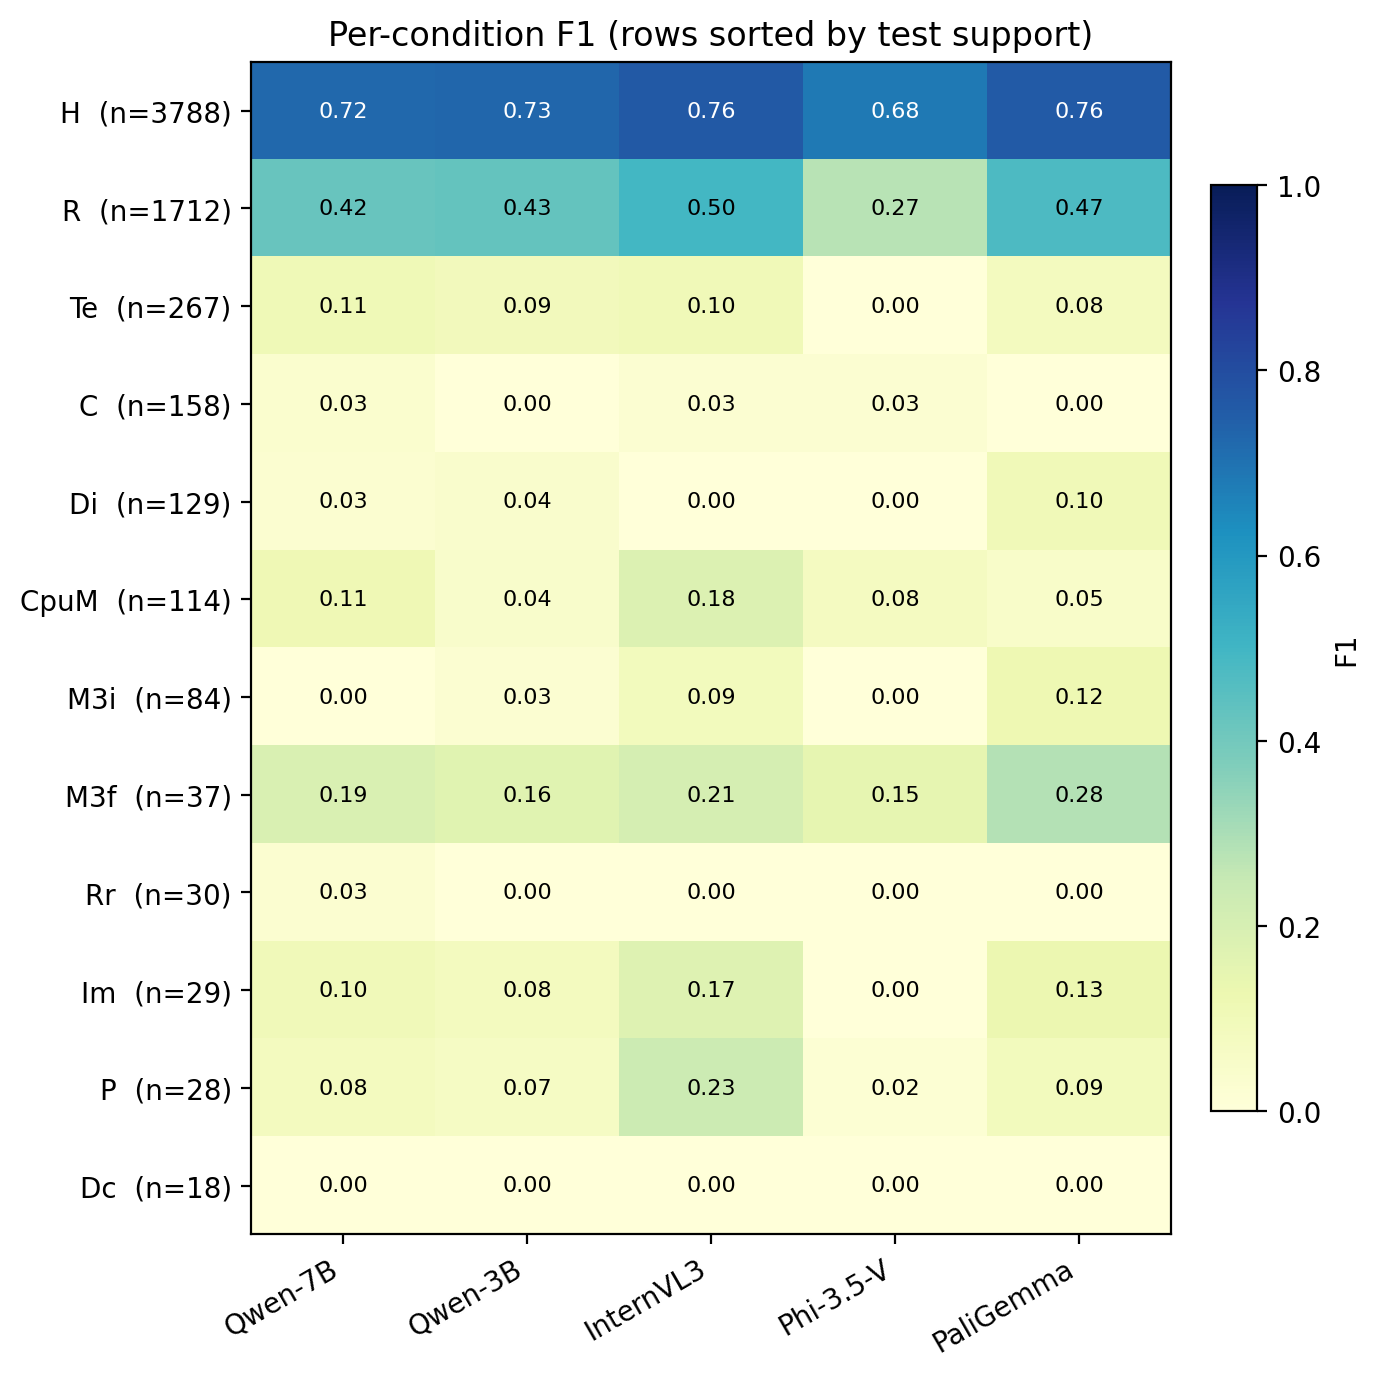
\includegraphics[width=0.85\textwidth]{per_condition_heatmap.png}
    \caption{Per-condition F1 for every model, with the conditions sorted by test support (the count is shown next to each row). The two common conditions (\texttt{H}, \texttt{R}) are read well by all models, while the rare conditions stay close to zero. This view makes the effect of the class imbalance easy to see.}
    \label{fig:per-condition-heatmap}
\end{figure}

\section{Effect of the Imbalance Handling}

The training uses two techniques against the class imbalance: oversampling the rare-condition rows (Section~\ref{sec:materials}) and up-weighting the loss on the rare-condition tokens (Section~\ref{sec:loss-weighting}). Their effect is read from the rare-condition rows of Table~\ref{tab:results-percond} and from the macro F1 in Table~\ref{tab:results-recognition}. A model that ignored the rare conditions would score near zero on those rows and would have a low macro F1, even with a high micro F1.

With the imbalance handling in place, the rare conditions are not fully ignored. Three of the five rare conditions (\texttt{M3f}, \texttt{P}, and \texttt{Im}) reach a non-zero F1 for most models, and the macro F1 stays in the 0.10 to 0.19 range instead of collapsing to near zero. The strongest case is \texttt{M3f}, which reaches a recall above 0.7 for every model. So the two techniques do move the rare conditions away from a pure ``label everything healthy'' result.

The effect is still limited. Two rare conditions, crown destruction (\texttt{Dc}) and residual root (\texttt{Rr}), stay near zero for almost every model. These two have the fewest test teeth (18 and 30), and the visual sign is small, so the extra signal from oversampling and loss weighting was not enough. The high recall but low precision on \texttt{M3f} also shows a cost: the model now over-predicts the conditions that were pushed harder. A controlled ablation, with one run using neither technique, would measure the exact gain. That run is not available here, so the effect is read only from the rare-condition rows and the macro F1, and the conclusion is kept modest: the handling helps the easier rare conditions, but the rarest and the visually small ones remain unsolved.

\section{Per-Tooth Detection}

Figure~\ref{fig:fdi-chart} shows the per-tooth detection recall for the best model, laid out like a dental chart. A greener cell means the tooth at that FDI position is found more often, and a redder cell means it is missed more often. This view shows whether the misses are spread evenly or concentrated on certain positions, such as the wisdom teeth at the back of the mouth.

\begin{figure}[H]
    \centering
    % Produced by visualize.py as fdi_recall_chart_<model>.png
    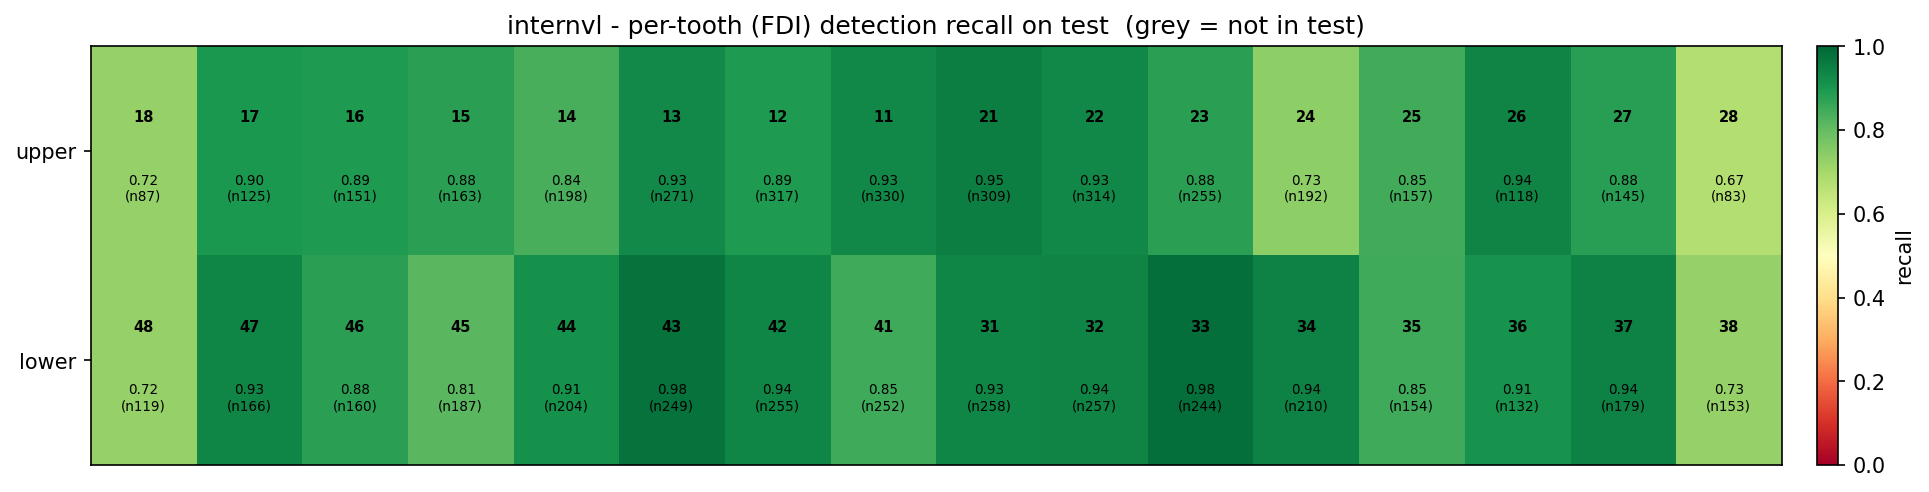
\includegraphics[width=\textwidth]{fdi_recall_chart_internvl.png}
    \caption{Per-tooth (FDI) detection recall on the test set for the best model. The upper jaw is on top and the lower jaw on the bottom; each cell shows the recall and the test count for that tooth.}
    \label{fig:fdi-chart}
\end{figure}

For InternVL3, the best model, the misses are not spread evenly. The lowest recall is on the four wisdom teeth, at FDI positions 18, 28, 38, and 48. Their recall is about 0.67 to 0.73, while most front and middle teeth are above 0.85. The upper-left wisdom tooth (28) is the worst, found in only about two thirds of the cases.

This matches the expectation. The wisdom teeth sit at the very back of the mouth. They are often missing, already removed, or still under the gum, and on a panoramic image their region is the most crowded and the least clear. So a lower recall there is reasonable. It also means the misses are concentrated in a small, explainable group of teeth, not scattered at random across the mouth.

\section{Confusion Analysis}

Figure~\ref{fig:confusion} shows the confusion matrix between the gold and the predicted conditions for the best model, normalised by row so the diagonal is the recall of each condition. The off-diagonal cells show the typical mistakes, for example a rare condition being predicted as healthy or restored.

\begin{figure}[H]
    \centering
    % Produced by visualize.py as cm_norm_<model>.png
    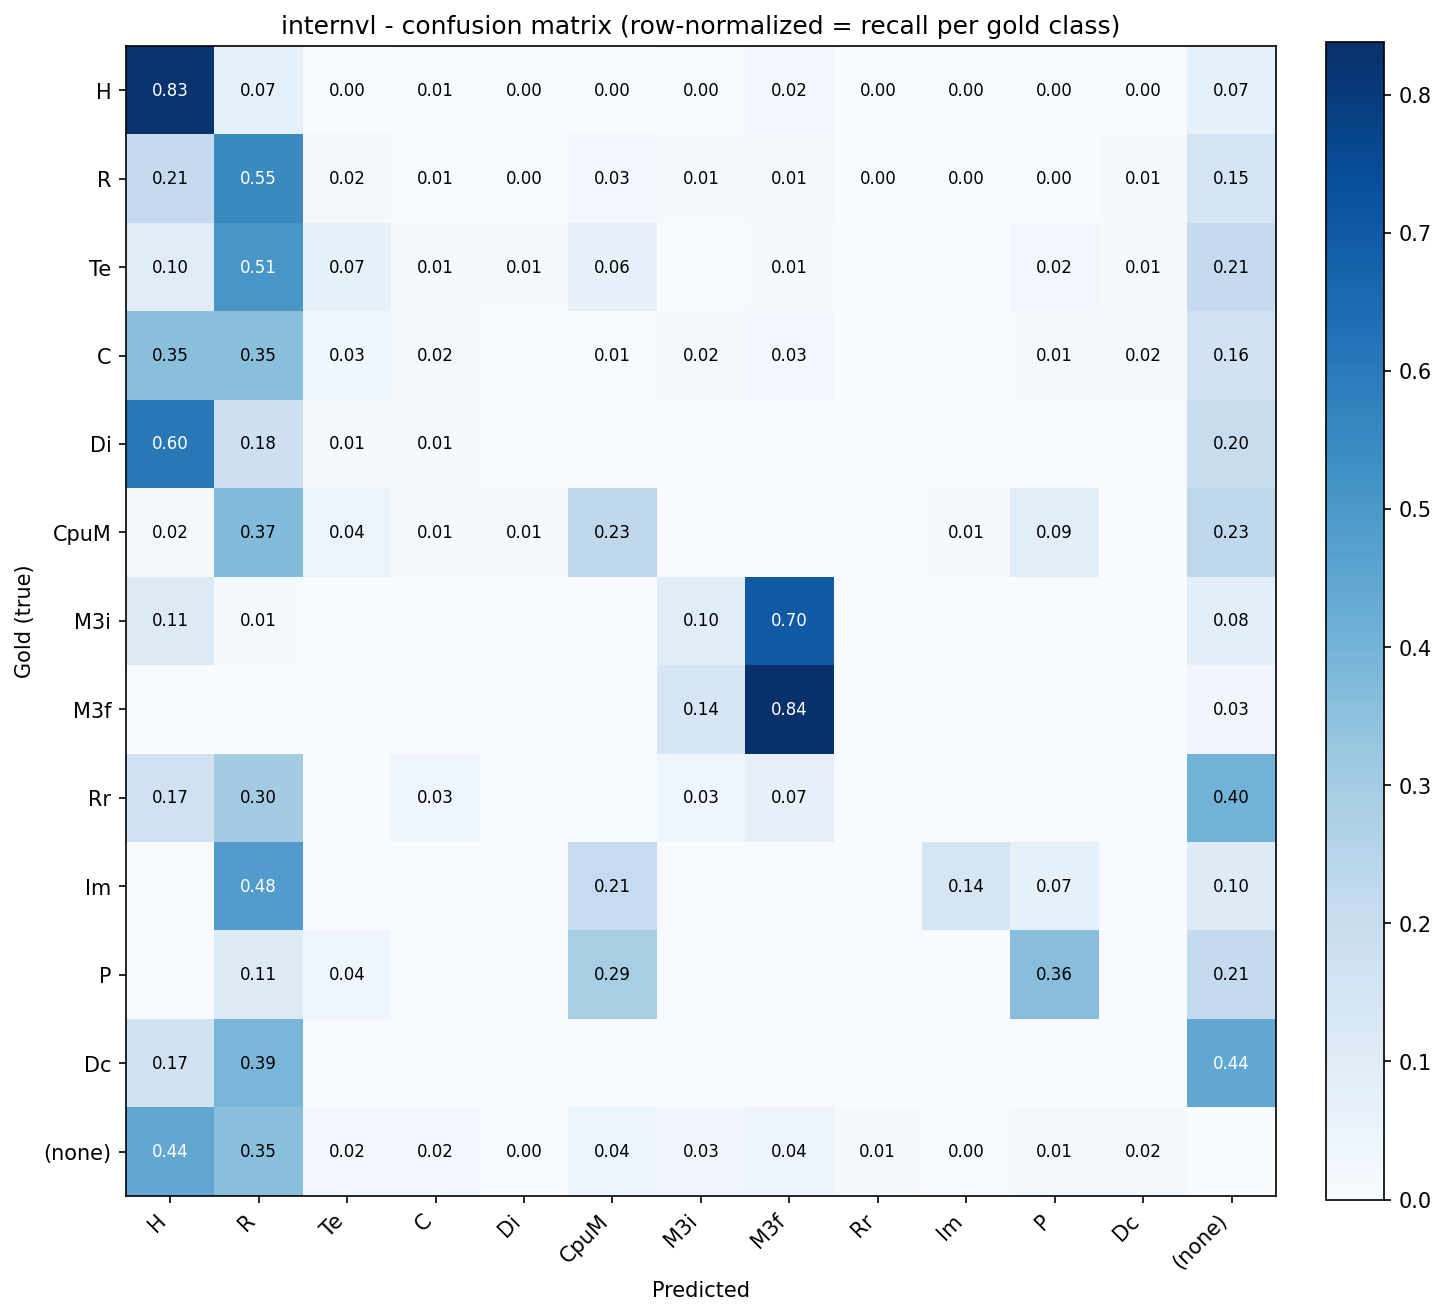
\includegraphics[width=0.9\textwidth]{cm_norm_internvl.png}
    \caption{Row-normalised confusion matrix of conditions for the best model. The diagonal is the per-condition recall; bright off-diagonal cells are common mistakes.}
    \label{fig:confusion}
\end{figure}

For InternVL3, the most common mistakes are between the two common classes and from a rare class into a common one. The largest single confusion is restored predicted as healthy (364 teeth), followed by healthy predicted as restored (261 teeth). So the model often mixes up \texttt{H} and \texttt{R}, which look similar on the image. After that, endodontic treatment is predicted as restored (\texttt{Te} to \texttt{R}, 135 teeth), and incisal or occlusal wear is predicted as healthy (\texttt{Di} to \texttt{H}, 78 teeth).

The pattern is clear: when the model is wrong on a less common condition, it usually falls back to healthy or restored, the two classes it has seen most. This is the expected effect of the class imbalance. One confusion goes the other way, healthy predicted as developing third molar (\texttt{H} to \texttt{M3f}, 76 teeth). This is the over-prediction of \texttt{M3f} seen earlier, and it comes from pushing that rare class harder during training.

\section{Qualitative Example}

Table~\ref{tab:qualitative} places one gold report next to the InternVL3 prediction for the same image, so the output can be judged by eye and not only by the metrics. The example is the lower-left region of one test image.

\begin{table}[H]
\centering
\caption{One gold report and the InternVL3 prediction for the same test image (lower-left region). The \texttt{condition\_name} field is left out to save space.}
\label{tab:qualitative}
\begin{tabular}{p{6cm}p{6cm}}
\toprule
Gold report & Model prediction (InternVL3) \\
\midrule
{\ttfamily\footnotesize
\{"region":"image\_lower\_left",\newline
"teeth":[\newline
\{"fdi":"32","condition":"Di"\},\newline
\{"fdi":"33","condition":"R"\},\newline
\{"fdi":"43","condition":"R"\},\newline
\{"fdi":"44","condition":"R"\},\newline
\{"fdi":"45","condition":"H"\}],\newline
"comment":"This region shows incisal or occlusal wear on tooth 32, and restorations on teeth 33, 43, and 44. The remaining annotated teeth are healthy."\}
}
&
{\ttfamily\footnotesize
\{"region":"image\_lower\_left",\newline
"teeth":[\newline
\{"fdi":"33","condition":"R"\},\newline
\{"fdi":"43","condition":"R"\}],\newline
"comment":"This region shows restorations on teeth 33 and 43."\}
}
\\
\bottomrule
\end{tabular}
\end{table}

The example shows the typical behaviour of the model. The teeth it does report are correct: 33 and 43 are both restored in the gold report, and the comment text is clean and well formed. But the model misses three teeth. It does not report tooth 44 (restored), tooth 45 (healthy), or tooth 32, which has the rare condition of incisal or occlusal wear. This is the same pattern seen in the metrics: the model finds and names some teeth correctly, but it tends to miss teeth, and it misses the rare condition rather than guessing it.

\section{Comparison with a Faster R-CNN Baseline}
\label{sec:frcnn-compare}

The same dental data was also used to train a Faster R-CNN detector, as a recognition baseline. The detector follows a standard object-detection setup. It is trained on COCO-style boxes with a ResNet50 backbone, and it is scored with detection metrics. Two separate detectors are built: one predicts the FDI tooth number, and one predicts the condition. Table~\ref{tab:frcnn-compare} places the best VLM next to the best Faster R-CNN.

\begin{table}[H]
\centering
\caption{Best VLM versus best Faster R-CNN on tooth detection (FDI) and condition classification. The two systems use different test splits and different matching rules, so the numbers are indicative, not a controlled head-to-head.}
\label{tab:frcnn-compare}
\begin{tabular}{llcc}
\toprule
Task & Metric & Best VLM (InternVL3) & Best Faster R-CNN \\
\midrule
\multirow{3}{*}{Detection (FDI)} & Precision   & 0.776 & \textbf{0.818} \\
                                 & Recall      & 0.892 & \textbf{0.964} \\
                                 & F1          & 0.830 & \textbf{0.885} \\
\midrule
\multirow{3}{*}{Classification}  & Micro F1    & 0.607 & \textbf{0.860} \\
                                 & Macro F1    & 0.189 & \textbf{0.601} \\
                                 & Weighted F1 & 0.598 & \textbf{0.864} \\
\bottomrule
\end{tabular}
\end{table}

The comparison must be read with care, because the two systems are not measured on the same ground. The detector uses a different test split, with 120 images and empty images removed, while the VLM uses 93 images in five views each. The matching rule is also different. The detector counts a tooth as found when the predicted box overlaps the gold box (IoU), while the VLM counts a tooth by an exact match of its region and FDI number. So the numbers are indicative, not an exact head-to-head.

With that in mind, the result is clear. Faster R-CNN is stronger at recognition. It detects teeth better (FDI F1 0.885 against 0.830), and it classifies the condition far better (macro F1 0.601 against 0.189). The gap is largest on the rare conditions, which the detector keeps well above zero while the VLM often drops to zero. This fits the design of the two systems. The detector treats every tooth as an equal target with a clean box-level signal, so a rare condition is not washed out. The VLM is trained with a token-level loss, where a rare condition code is only a few tokens in a long report, so the rare signal stays weak.

But the two systems do different jobs. The detector outputs boxes and labels only, and it uses two separate models that do not link which condition sits on which tooth. The VLM produces one structured report that lists each tooth, its condition, and a short comment together. So the Faster R-CNN result is best read as a recognition ceiling for this data. It shows how much accuracy a specialist detector can reach, while the VLM trades some of that accuracy for a readable, report-style output.

\section{Discussion}

The results give a clear picture of what works on this task and what does not.

The best model is InternVL3-8B. It leads on macro F1, micro F1, and tooth accuracy, and it has a clean output with 100\% valid JSON. PaliGemma~2 is the close second, and this is the most interesting result. PaliGemma~2 is the smallest model in the set, about 3B, and it uses a fixed 448-pixel image. Yet it almost matches an 8B model, and it has the lowest miss rate and the highest ROUGE-L. So for this task, a careful smaller model is enough, and a fixed image size is not a real handicap.

This leads to the first conclusion: model size is not the main factor here. The 3B PaliGemma~2 matches the 8B InternVL3, and the 3B Qwen matches or slightly beats the 7B Qwen. The 7B Qwen only has a small edge on macro F1, which means it handles the rare conditions a little better. For a small, structured task like this one, the extra parameters of a larger model are mostly wasted. The architecture and the encoder matter more than the parameter count.

The vision encoder is the most likely reason for the ranking. InternVL3 uses InternViT-300M, and PaliGemma~2 uses SigLIP-So400m. Both are strong vision encoders trained on very large image data, and PaliGemma~2 is also pretrained on grounded tasks such as detection and captioning. These two models take the first and second place. Phi-3.5-vision uses an older CLIP ViT-L/14 encoder, and it is last on every metric. The two Qwen models sit in the middle and score almost the same, which again shows that the language-model size is not the bottleneck. So on this task, the quality of the vision encoder, not the parameter count, explains most of the difference between the models.

The second conclusion is about where the models fail. Detection is not the problem. Every model finds the teeth with an FDI F1 of about 0.80 to 0.83. The problem is the condition. The tooth accuracy drops to 0.38 to 0.52, and the macro F1 stays near 0.10 to 0.19. The main error type is therefore a wrong or missing condition, not an invented tooth. The confusion analysis confirms this: a rare condition is usually predicted as healthy or restored, the two common classes.

The third conclusion is about the class imbalance. The two techniques, oversampling and rare-token loss weighting, do help. They keep several rare conditions above zero and stop the model from labelling every tooth as healthy. But the help is limited. The rarest conditions, crown destruction and residual root, stay near zero, and even caries, which is not rare, is almost never read correctly. The handling also has a cost: the model now over-predicts the conditions it was pushed to learn, such as developing third molar. So the imbalance is reduced but not solved.

The Faster R-CNN baseline in Section~\ref{sec:frcnn-compare} shows that this is not only a data limit. A specialist detector reaches a much higher rare-condition score on the same data. So a large part of the gap comes from the report-generation approach itself, where the rare codes are weak in the token-level loss, and not only from the class imbalance.

These results fit the goal of the thesis. The output is meant to be a first draft, not a final diagnosis. As a first draft, the models are useful for the common findings: they find most teeth and read healthy and restored teeth fairly well. They are not yet reliable for the rare conditions, and caries is a clear weak point. For this reason, the generated report still needs a dentist to check it, especially for the rare and the small findings. The work shows that vision-language models can produce a structured dental report, but it also shows that the rare-condition recognition is the open problem for future work.

% --- Appendix starts ---
\appendix
\chapter{Prompts}\label{app:prompts}

\section*{Prompt Template for Full Panoramic Report}\label{app:full-report-prompt}

\begin{lstlisting}[style=mystyle,numbers=none, caption={Prompt template for full panoramic dental report},label={lst:full-report-prompt}]
<image>
This is a full panoramic dental radiograph.
Divide the image into four image-space regions: image_upper_left, image_upper_right, image_lower_left, and image_lower_right.
For each region, list the visible annotated teeth using FDI notation and report each tooth condition.
Return only valid JSON with this schema:
{"regions":{"image_upper_left":{"teeth":[{"fdi":"string","condition":"string","condition_name":"string"}],"comment":"string"},"image_upper_right":{"teeth":[{"fdi":"string","condition":"string","condition_name":"string"}],"comment":"string"},"image_lower_left":{"teeth":[{"fdi":"string","condition":"string","condition_name":"string"}],"comment":"string"},"image_lower_right":{"teeth":[{"fdi":"string","condition":"string","condition_name":"string"}],"comment":"string"}},"summary":"string"}
\end{lstlisting}

\section*{Prompt Template for Regional Report}\label{app:regional-report-prompt}

\begin{lstlisting}[style=mystyle,numbers=none, caption={Prompt template for regional dental report},label={lst:regional-report-prompt}]
<image>
This is the {region} crop of a panoramic dental radiograph.
Identify the visible annotated teeth using FDI notation and report each tooth condition.
Return only valid JSON with this schema:
{"region":"string","teeth":[{"fdi":"string","condition":"string","condition_name":"string"}],"comment":"string"}
\end{lstlisting}


\bibliographystyle{IEEEtran}
\bibliography{references}




\end{document}
